%\documentclass[12pt,ascmac]{jreport}
\documentclass[12pt]{jreport}
\usepackage{comment}
\usepackage{listings}
\usepackage{amsmath}
\usepackage{./sty/eclepsf}
\usepackage{tascmac}
\usepackage{tabularx}
\usepackage{listliketab}
\usepackage[longnamesfirst]{natbib}
\usepackage[dvipdfmx]{graphics}
\usepackage[dvipdfmx]{graphicx}
\usepackage[dvipdfmx]{color}
\usepackage{subfigure}
\usepackage{alltt}
\usepackage{here}
\usepackage{afterpage}
\usepackage{./sty/ncodeline}
\usepackage{longtable}
%\usepackage[textwidth=160mm, textheight=225mm]{geometry}
%\usepackage[dvipdfmx, colorlinks, breaklinks,%
\usepackage[dvipdfmx, breaklinks,%
bookmarks=true, bookmarksnumbered=true,%
bookmarkstype=toc, bookmarksopen=true,bookmarksopenlevel=3,%
pdftitle={Approximation of high-interaction honeypots by Command Extension of low-interaction honeypot},%
%%pdfsubject={},%
pdfauthor={Yuta Sugafuji},%
pdfkeywords={1.Natural Language Processing, 2.Semantic analysis, 3.Honeypot, 4.SSH}%
]{hyperref}
\usepackage{bookmark}

\AtBeginDvi{\special{pdf:tounicode EUC-UCS2}}

\usepackage{fancyhdr}

\usepackage{./sty/doxygenorig}

\usepackage{indentfirst}
\usepackage{url}
\usepackage{listings,./sty/jlisting}

\def\lstlistingname{プログラム}

\lstset{%
 language={C++},
 %backgroundcolor={\color[gray]{.85}},%
 basicstyle={\small\ttfamily},%
 identifierstyle={\small},%
 commentstyle={\small\itshape},%
 keywordstyle={\small\bfseries},%
 ndkeywordstyle={\small\ttfamily},%
 stringstyle={\small\ttfamily},
 frame={tb},
 framesep=1zw,
 breaklines=true,
 numbers=left,%
 xrightmargin=0zw,%
 xleftmargin=1.5zw,%
 numberstyle={\scriptsize},%
 stepnumber=1,
 numbersep=1zw,%
 lineskip=-0.5ex%
}

\usepackage{amssymb}
%\usepackage{supertabular,multirow}

\usepackage{array}
\newcolumntype{M}[1]{>{\centering\arraybackslash}m{#1}}

% A4  size: 297mm*210mm %1pt = 0.35mm
\setlength{\topmargin}{-3.4mm} % 10pt 25.4mm - 3.4mm = 22mm
\setlength{\oddsidemargin}{-0.4mm} % 25.4mm - 0.4mm = 25mm
\setlength{\evensidemargin}{-0.4mm} % 25.4mm - 0.4mm = 25mm
\setlength{\textheight}{231mm} % 660pt % original is 225.75mm 645pt
\setlength{\textwidth}{160mm} % 457pt

\renewcommand{\topfraction}{.99}
\renewcommand{\textfraction}{.0}
\renewcommand{\floatpagefraction}{.99}
\renewcommand{\bibname}{参考文献}


\pagestyle{fancy}
%\rhead{\thepage}
%\rhead[]{\leftmark}
\lhead[]{}
%\lhead[\rightmark]{}

\makeatletter
\def\chaptermark#1{\markboth {\ifnum \c@secnumdepth>\m@ne
\@chapapp\ \thechapter \@chappos\ \fi #1}{}}
\makeatother

\newcommand{\bbc}{Bitcoin Blockchain}
\newcommand{\ebc}{Ethereum Blockchain}
\makeatletter
\newcommand{\subsubsubsection}{\@startsection{paragraph}{4}{\z@}%
  {1.0\Cvs \@plus.5\Cdp \@minus.2\Cdp}%
  {.1\Cvs \@plus.3\Cdp}%
  {\reset@font\sffamily\normalsize}
}
\makeatother
\setcounter{secnumdepth}{4}

\begin{document}

\pagenumbering{roman}
\begin{titlepage}
  \begin{center}
    \begin{large}
      卒業論文   2018年度(平成30年)\\
      \vspace{24pt}
      低対話型Honeypotのコマンド拡張による\\高対話型Honeypotへの近似
      \end{large}
  \end{center}
  \vspace{40em}
  \begin{flushright}
    \large 慶應義塾大学 総合政策学部\\
    菅藤 佑太
  \end{flushright}
\end{titlepage}

\thispagestyle{empty}


卒業論文要旨 - 2018年度 (平成30年度)
\begin{center}
\begin{large}
\begin{tabular}{|M{0.97\linewidth}|}
    \hline
   低対話型Honeypotのコマンド拡張による\\高対話型Honeypotへの近似\\
    \hline
\end{tabular}
\end{large}
\end{center}

~ \\

PCの普及やIoTデバイスのシステム高度化により,高度な処理系を組むことが可能になった.これによりデバイス上にLinux系などのOSが搭載された機器が広く人々に使われるようになった.また,Linux系OSにリモートログインする手法としてSSHがある.これを用いて不正に侵入する攻撃が行われている.
侵入された際に侵入者がどのような挙動をしているのかを知る手段として,Honeypotがある.HoneypotはSSHで侵入しやすいような環境を作ることで,侵入者にログイン試行に成功したと検知させ,その際に実行したコマンドのログを収集するものである.また現在ではShellの挙動をエミュレートしたHoneypotが広く使用されており,このHoneypotは実行できるコマンドが少ない実装になっている.そのためHoneypotへの侵入者に侵入先がHoneypotであると検知されてしまう.そこで事前実験ではHoneypotのコマンドを拡張し,拡張をしていないHoneypotとコマンドの拡張をしたHoneypotで侵入ログを収集した.収集したログを確率的な算出方法を使用することで比較した結果,より多くの侵入者のコマンド実行ログのパターンを取得できることを示した.本研究ではコマンドを拡張したHoneypotの侵入ログがどれほど実際のOSに不正なSSHの侵入をされた際の侵入ログの近似を試みた.評価として,拡張をしていないHoneypotとコマンドの拡張をしたHoneypotと,さらに実際のOSを使用したHoneypotで侵入ログを収集し,比較を行なった.この3つの侵入ログを自然言語処理の意味解析を用い,コマンドの一つ一つの意味をベクトル表現することで,拡張したHoneypotで収集した侵入ログが,拡張をしていないHoneypotで収集した侵入ログよりも,実際のOSを使用したHoneypotで侵入ログに意味的に近くなることが明らかとなった.


~ \\
キーワード:\\
\underline{1. SSH},
\underline{2. Honeypot},
\underline{3. 機械学習},
\underline{4. 自然言語処理}
\begin{flushright}
慶應義塾大学 総合政策学部\\
菅藤 佑太
\end{flushright}

\thispagestyle{plain}
\clearpage

Abstract of Bachelor's Thesis - Academic Year 2018
\begin{center}
\begin{large}
\begin{tabular}{|p{0.97\linewidth}|}
    \hline
        Approximation of high-interaction honeypots\\
by Command Extension of low-interaction honeypot\\
    \hline
\end{tabular}
\end{large}
\end{center}

~ \\
\renewcommand{\baselinestretch}{0.9}
I was able to make high processing system, and a moving apparatus is wide, and the OS's such as the Linux system came to be in this way used for people on a device, and, meanwhile, one's apparatus is stepped over by an unjust invasion of SSH, and I am attacked to the network apparatus of the third party from an apparatus of oneself by the spread of PCs and the system advancement of the IoT device, and a problem made in the environment that a virus and a back door are installed, and is carried out a virus an apparatus of oneself illegally occurs.
Let an intruder detect it by making the environment that there is ,Honeypot as a window what kind of ways an intruder behaves when was invaded, and is easy to invade it daringly in SSH when succeeded in a login trial, and Honeypot which collect the log of the command that carried out on this occasion, and emulated behavior of Shell now again is wide, and is used, and there are few commands that this Honeypot can carry out; showed that could acquire a pattern of the command practice log of more intruders by being implemented, and therefore being detected by an intruder to Honeypot when invasion ahead was Honeypot, and expanding the command of Honeypot by a there prior experiment, and evaluated it using natural language processing whether invasion log of Honeypot which expanded the command in this study was similar to invasion log when was invaded of SSH which was how unjust for the real OS.
\renewcommand{\baselinestretch}{1.0}

~ \\
Keywords : \\
\underline{1. SSH},
\underline{2. Honeypot},
\underline{3. Machine Learning},
\underline{4. Natural Language Processing}
\begin{flushright}
Keio University, Faculty of Policy Management Studies\\
Yuta Sugafuji
\end{flushright}

\thispagestyle{plain}
\clearpage

\tableofcontents\thispagestyle{plain} %目次
\clearpage
\listoffigures\thispagestyle{plain} %図目次
\clearpage
\listoftables\thispagestyle{plain} %表目次
\clearpage

\pagenumbering{arabic}
\chapter{序論}
\label{introduction}

本章では本研究の背景,課題及び手法を提示し,本研究の概要を示す.

\subsection{研究の背景}
\label{introduction:haikei}

PCの普及やIoTデバイスのシステム高度化により,高度な処理系を組むことが可能になり,デバイス上にLinux系などのOSが動く機器が広く人々に使われるようになった.そうした中でSSHの攻撃によって自分の機器が踏み台にされ,自身の機器から第三者のネットワーク機器に攻撃されていたり,ウイルスやバックドアが設置されて自身の機器が不正にウイルスが実行されるような環境を作られる問題が発生している.\\
 侵入された際に侵入者がどのような挙動をしているのかを知る手段として,Honeypotというものがある.これはShellの擬似的な挙動をアプリケーション上で実現し,敢えてSSHで侵入しやすいような環境を作ることで,侵入者にログイン試行に成功したと検知させ,その際に実行したコマンドのログを収集する.\\
\ \ SSHのHoneypotは大きく二種類に分けることができ,一つは低対話型Honeypot,もう一つは高対話型Honeypotである.低対話型Honeypotは実際のShellの挙動をエミュレートしたアプリケーションシステムである.高対話型Honeypotは他のホストに攻撃しないようにネットワークの設定を適切に行い,またrootの権限が取られないようにuser権限を適切に行ったりするなどの設定を施した実際のOSを用いた仕組みである.高対話型Honeypotは低対話型Honeypotと比較すると,本物のOSを用いている分高精度な攻撃ログを取得することができるが,乗っ取られ他のホストに攻撃をしたりウイルスに犯されてしまうなどの危険を孕んでいるため設置コストが高く,普及率も非常に低い.一方で低対話型Honeypotはアプリケーションシステムであるため,root権限を取られるような危険が極めて少なく,アプリケーションシステム内での脆弱性だけに限った問題しか存在しない.そのため設置コストが低く,ドキュメントが多く存在し比較的誰でも安全に設置できるため,普及率が高い.しかし,実際のShellとは異なる挙動や,Honeypotに特有な挙動をしてしまうため,設置したHoneypotに侵入した悪意のあるユーザーに侵入先がHoneypotであると検知されてしまう可能性がある.\\
\ \ この低対話型Honeypotの設置コストの低さで,かつHoneypotに侵入してきた悪意のあるユーザーに侵入先がHoneypotであると検知されないように攻撃ログを取得するためには,低対話型Honeypotの挙動をできるだけ実際のShellに近似すれば良いのではないかと考えられる.\\
\ \ 本研究の予備実験では,SSHの低対話型Honeypotに実装されていないコマンドで悪意のある侵入者が使うようなコマンドを実装し,何の追加実装も施していないSSHの低対話型Honeypotで取れた侵入者の実行コマンドログと ,追加実装を施したSSHの低対話型Honeypotの侵入者の実行コマンドログを比較することで,追加実装を施したSSHの低対話型Honeypotの方がコマンドパターンとして多く収集できることを示した.\\
\ \ 本研究では低対話型Honeypotを実際のShellの挙動に近似するために,実際のShellに実装されているもので低対話型Honeypotに実装されていないコマンドの実装や,低対話型Honeypotに特有の異常な挙動を修正を行いこの問題を解決できるのではないかと考えた.\\
\ \ 実際のShellの挙動に近似するように実装した低対話型Honeypotで取れた攻撃ログが,何の実装を施していない純正の低対話型Honeypotで取れた攻撃ログと比較して,実際のOSで用いた攻撃ログにどれほど近しいかを時系列データを教師データとした機械学習を用いて検証することで評価した.

%\section{デジタルファブリケーションの発達}
%\label{introduction:background}

%本節では,デジタルファブリケーションと呼ばれるものづくりの発達と,それに伴うパーソナルファブリケーションについて説明する.

%\section{デジタルファブリケーション}
%\label{introduction:digitalfabrication}

%デジタルファブリケーションとは,3Dプリンタやレーザカッタといったコンピュータに接続されたデジタル工作機器を用いて3Dモデルを実際に造形物として成形する技術のことである.近年,コンピュータの普及とともに,デジタル工作機器は安価かつ小型になりつつある.また3Dモデリングソフトウェアもオープンソースのものが現れるなど,個人であっても高精度で3Dモデルを出力できる機器を入手,製造が行える環境ができつつある.


%\subsection{3Dプリントの普及と活用}
%\label{introduction:3dprintrise}
%2000年代後半以降,技術の発達や低コスト化により,3Dプリンタが急速に普及している。3Dプリンタは樹脂素材などを加工し,設計図である3Dモデル同様の立体物を造形するデジタル工作機器である.1980年代の開発当初3Dプリンタは工業製品の試作のために製造業の中で主に使われていた.2005年にアメリカの3D Systems社が保持していた光造形法をはじめとする多くの造形手法が特許失効したことや,3Dプリンタ自体の製造技術の発達などの理由で,安価なものが作られるようになった.


%また,インターネット上で,3Dプリンタに関連する情報や,実際にプリントを行うための設計図などが,数多くWebで共有されている\cite{Thingiverse}.そうした情報を入手することで,今まで専門的な機器であった3Dプリンタを個人でも扱える環境が整いつつある.


%3Dプリンタの安価化と情報共有の迅速化・簡易化の二つの要因により,専門家以外による3Dプリンタを用いたものづくりは急速に普及している.3Dプリンタの市場規模は2015年の段階で11億ドルに対し,2019年には26億ドル超になると予測されている\cite{3dprintermarket}.そうした中で,現在Fablab\cite{FabLab}と呼ばれるデジタル工作機器を扱うことができる施設が世界各地で設置されており,デジタルファブリケーションの普及に努める拠点となっている.日本でも2010年以降神奈川県鎌倉市や茨城県つくば市を始めとして各地に設置されている.Fablabでは個人がデジタル工作機器を持たずとも,デジタルファブリケーションを行うことができる.


%3Dプリントの普及に伴い,開発当初想定されていた試作以外にも様々な応用が考えられるようになった.応用例の一つとして義足が挙げられる\cite{3dprintProstheticleg}.義足は使用者によってそのサイズや形状が異なるため,一律に大量生産することはできない.そのため,既存の義足の製作は,熟練した専門家によってオーダーメイドで制作されており,製作自体や修正も簡単ではない.3Dプリントであれば,3Dモデルを個人の形に合わせて改変することが容易である.修正する場合も,3Dモデルの修正と再出力は簡単に行うことができる.また,福田\cite{3dperson}は自分の実物大の3Dモデルを用いた作品を製作し,慶應義塾大学湘南藤沢キャンパス内で展示を行った.出力の際に3Dモデルの解像度を調整することで,作品の閲覧者が制作物から3Dモデルの元となった人物を特定できることをなどを確認した.これは芸術分野においても3Dモデルの改変や再出力によって様々な可能性があることを示唆するものである.

%\subsection{パーソナルファブリケーションとオープンデザイン}
%\label{introduction:personalfabrication}
%3Dプリンタの普及に伴い,個人で製造を行うパーソナルファブリケーションと呼ばれるものづくりも行なわれつつある\cite{mota2011rise}.インターネットを通じて入手した3Dモデルを自分の環境に合わせて改変しプリントを行うなど,3Dモデルの2次利用,3次利用も行なわれている.インターネット上で公開した3Dモデルが,他人によって改変され派生が生まれる中で,2次利用者が加えた改変が元の3Dモデルに取り入れられることもある.これは,ソフトウェア開発におけるオープンソースと似た構造である.これらの動きから,オープンソースの考え方などをデザインに適用する``オープンデザイン"という概念も提唱されている\cite{opendesign}.


%\section{本研究の着目する課題と目的}
%\label{introduction:issue}

%現在のデジタルファブリケーションでは個人で製造において,製造責任の追及や知的財産権の保証のために,製造物の製造情報の管理が一つの課題となっている.ここで扱う製造情報としては,設計図情報である3Dモデルデータ,3Dデータの設計者,製造者,製造日時などが含まれる.例えば,製造物によって事故が起こった場合,その責任を誰に求めるかといった製造責任(Product Liability,PL)の追求を行う.その際設計図などから設計上の欠陥を追及する必要性がある.また,自分の設計物を知的財産として証明する際にも製造情報が保存されていることが必要である.製造責任の追及や知的財産権の保障を行う為には,データが誰にでも参照できる公開性,製造物からデータが追跡できる追跡可能性,保存されたデータが後日改ざんされておらず完全性を保っていることが必要である.そこで,3Dプリントの際にRFIDを製造物に埋め込み,データサーバに保存された製造情報と製造物を紐付ける試みが行われている\cite{3dprintwithrfid}.この手法では,追跡可能性は担保されるものの,製造物に紐づけられた製造情報の完全性が担保されていない.


%本研究では,パーソナルファブリケーションによる個人的な製造が行われる中で,製造責任の知的財産権の所在を明らかにするシステムを提案した.

%\section{本研究の仮説}
%\label{introduction:hypothesis}

%Bitcoinの基幹技術として発明されたBlockchain技術は,P2Pネットワーク上でデータが検証されたことを合意し公開台帳を形成するシステムである.公開台帳上に記録されたデータは各参加ノードによって分散的に保持され,改ざんを相互に監視するため,正規の手続きを踏まなければデータの更新もできず,データが失われる可能性も極めて低い.

%そこで本研究では,3Dプリントにおける製造情報をBlockchain上に保存することで,~\ref{introduction:issue}節で述べた条件を満たし,製造責任や知的財産権の所在を明らかにできるのではないかと考えた.


%\section{本研究の手法}
%\label{introduction:method}
%本研究では,3Dプリンタを制御するシングルボードコンピュータをEthereumノードとすることでBlockchain上に製造情報を保存する実験システムを構築した.EthereumとはBlockchainを状態遷移を記録する公開台帳として用いるためのアプリケーション開発プラットフォームである.Blockchain上に製造情報を保存できていることを確認し,本システムのスケーラビリティ,情報の改ざん耐性を推定することで,要件を満たせることを確認した.


\section{本論文の構成}
\label{introduction:kosei}
本論文の構成を以下に示す.第1章では,本研究の背景と目的について述べた.第2章では,本研究の要素技術となるShellとHoneypotと時系列データの扱いについて整理する.第3章では本研究にあたっての事前実験の概要と結果を述べ,第4章では,本研究の問題の定義をする.第5章では,本提案手法のシステムについて解説する.第6章では,実装方法や実装例について述べ,第7章で提案システムの評価手法について説明する.第8章では先行研究や事例について紹介する.第9章では本研究のまとめと展望について言及する.
%本論文における以降の構成は次の通りである.

%~\ref{issue}章では,3Dプリント技術とそれに伴う法的課題とBlockchain技術に関して議論し,本研究の背景を明確化する.
%~\ref{approach}章では,本研究における問題の定義と,解決するための要件,仮説と手法について説明する.
%~\ref{implementation}章では,3Dプリンタをネットワークに接続させ制御し,Blockchainノードとすることで製造情報の保存をするシステムの実装を概説する.
%~\ref{evaluation}章では,\ref{issue}章で求められた課題に対しての評価を行い,考察する.
%~\ref{conclusion}章では,本研究のまとめと今後の課題についてまとめる.


%%% Local Variables:
%%% mode: japanese-latex
%%% TeX-master: "../thesis"
%%% End:

\chapter{本研究の要素技術}
\label{tech}

本章では,本研究の要素技術となるShellとHoneypotと時系列データの扱いについて各々整理する.

\section{Honeypot}

使われているデバイスへの不正なSSHによって侵入された際に,侵入者のログを収集する手段としてのHoneypotがある.SSHのHoneypot\cite{honeypot}は低対話型Honeypotと高対話型Honeypotの大きく二種類に分けることができる.\\
%以下に侵入者がSSHで不正に機器に侵入してから踏み台にして他の機器に攻撃を仕掛けるまでの一般的なフローを図2に示す.
%\vspace{10mm}
%\begin{figure}[H]
%    \centering
%    \includegraphics[width=1.0\textwidth]{figures/nagare.png}
%    \caption{不正なSSH侵入者の想定行動フロー}
%    \label{fig:evo}
%\end{figure}


\subsection{低対話型Honeypot}
\label{tech:LowInteractionHoneypot}

SSHの低対話型Honeypotは実際のShellの挙動をエミュレートしたアプリケーションである.実際のShellの挙動をエミュレートしただけのアプリケーションなので,脆弱性がアプリケーション内に限られる.そのため,root権限を侵入者に許してしまい,踏み台にされてしまうなどの危険が極めて少ない.しかし,エミュレーションには限界があるため,コマンドやその挙動について,実際のShellとは異なる挙動をすることがある.そのため,侵入者に侵入先がHoneypotであると検知されてしまう.検知されることで,攻撃者は実際の攻撃を行わず,本来取れるはずの攻撃ログが収集できない可能性を含んでいる.そのため,収集ログの精度に問題がある.

\subsubsection{Kippo}
\label{tech:Kippo}

Kippoは,悪意のあるSSHのログイン試行者や侵入者の挙動やログを記録するために使用されるPythonで実装されたSSHの低対話型Honeypotである\cite{kippo}.Kippoは前身のKojoney\cite{kojoney}に大きく影響を受けている.ネットワークはTwisted\cite{twisted}というフレームワークで組まれている.Kippoのプロジェクトは低対話型Honeypotとして2009年に登場し,Raspberry Pi\cite{rasp}などを筆頭としたシングルボードコンピュータ\cite{singleboard}の普及と相まって広く設置された.
Kippoの機能の特徴としては収集したコマンドログ を時系列データとして保存されており,"playlog"というKippo内にあるプログラムを実行することで,過去のコマンドログ を実際にタイピングしてるかのように出力できる.また,侵入者によってダウンロードされたファイルも実行ができないように保存できる.KippoはCowrieの登場によって2014年頃を最後に現在はプロジェクトが進んでいない.\cite{kippowiki}
KippoはIoTデバイスの高度化広く設置されたSSHの低対話型Honeypotのうちの一つであったが,実装されているコマンドも17\cite{kippocommand}と少なく,またKippo特有の異常な挙動が存在するなどと多くの問題があった.

\subsubsection{Cowrie}
\label{tech:Cowrie}
CowrieはPythonで実装されたSSHの低対話型Honeypotであり,実装はKippoのコマンドの拡張や攻撃者がリダイレクトでマルウェアを送り込む手法をとって送り込んだマルウェアを収集可能にしたりするなど,様々な機能を拡張したものとなっている.
Kippo特有の異常な挙動を改善しており,実装コマンド数は38\cite{cowriecommand}とKippoより少し多くなっているものの\cite{differfromkippo},Cowrie特有の異常な挙動もまだまだ多い.

%\subsection{製造責任と知的財産権に関する法制度}
%\label{tech:lows}


\subsection{高対話型Honeypot}
\label{tech:HighInteractionHoneypot}

\subsubsection{Honeynet Project}
\label{tech:Honeynet}

\subsection{SSHのHoneypotの比較}
\label{tech:CompareHoneypot}
以上をまとめたSSHの低対話型HoneypotとSSHの高対話型Honeypotの比較を行った表を図2に示す.

\vspace{10mm}
\begin{figure}[H]
    \centering
    \includegraphics[width=1.0\textwidth]{figures/compare.png}
    \caption{SSHの低対話型HoneypotとSSHの高対話型Honeypotの比較}
    \label{fig:evo}
\end{figure}

%\begin{itemize}
%\setlength{\leftskip}{1.0cm}
% \item[危険責任] 製造者は製造物の設計図などの情報を消費者より詳細に知り得るため
% \item[報償責任] 製造者は製造物により利益を得るためそこから生じる責任を負うべきである
% \item[信頼責任] 製造者は自己の製品の安全性についてPRしており消費者はその品質が担保されているものであると期待する
%\end{itemize}

\subsection{Shell}
\label{tech:Shell}
ShellはOSのユーザーのためにインタフェースで,カーネルのサービスへのアクセスを提供するソフトウェアである.本研究での"Shell"はコマンドラインシェルのことについてのことを指す.

\subsubsection{Secure Shell}
\label{tech:Secure Shell}
Secure Shell(セキュアシェル、SSH)は、暗号や認証の技術を利用して、安全にリモートコンピュータと通信するためのプロトコルである.パスワードなどの認証部分を含むすべてのネットワーク上の通信が暗号化される.\cite{ssh}SSHにおける問題としては,通信する上での認証方法には鍵認証を推奨されているが,デフォルトではパスワード認証になっている.また,パスワード認証のままだとパスワードの総当たり攻撃を受けたり,パスワードが標準のままの設定になっていることで不正なログイン試行によって侵入を許してしまう.

\subsubsection{BusyBox}
\label{tech:BusyBox}
BusyBoxは標準UNIXコマンドで重要な多数のプログラムを単一のバイナリファイルに含むプログラムである.BusyBoxに含まれる,多数の標準UNIXコマンドで必要とするプログラムの実行ファイルは,LinuxというOSをBusyBoxだけでディストリビューションできるよう,"Linux上で最小の実行ファイル"として設計されている.一般にインストールされる実行ファイルは一部だけを実装できるように選択することができる.一般的にはBusyBoxのコマンドは200以上も用意されている.\cite{busybox}\footnote{今回使用したBusyBoxに含まれるコマンドの数は219}.
このBusyBoxをインストールして実際にこれを実行するためには,BusyBox内にある各コマンドにアクセス可能なようにpathを通すだけで良い.

\subsection{自然言語処理}
\label{tech:NLP}
過去のデータの入力に対して未知のデータをどのようにして出力するのかについては様々な手法がある.本研究において自然言語処理は意味解析についてこれを使用した.

\subsubsection{統計的意味解析}
\label{tech:tokei}
過去のデータの入力に対して未知のデータを統計的に出力する.

\subsubsubsection{マルコフ連鎖}
\label{tech:Markov}

\subsubsubsection{コーパス}
\label{tech:Copus}

\subsubsubsection{シソーラス}
\label{tech:Siso}
シソーラス\cite{siso}

\subsubsection{ベクトル空間表現}
\label{tech:Vector}

\subsubsubsection{word2vec}
\label{tech:Word2vec}

%%% Local Variables:
%%% mode: japanese-latex
%%% TeX-master: "../bthesis"
%%% End:

\chapter{本研究における問題定義と仮説}
\label{approach}

本章では,~\ref{introduction}章で述べた背景より,本章では,現状のHoneypotの問題点を整理し,この問題をどのように解決すれば良いのかを定義する.

\section{本研究における問題定義}
\label{approach:problem}

\subsection{SSH\,Honeypotの現状の問題}
\label{approach:problemofSshHoneypot}
Honeypotには運用する上で大きな問題が2つある.一つは設置したHoneypotに悪意のある侵入者が侵入先をHoneypotであると検知してしまう問題である.もう一つはHoneypotに侵入を許した侵入者にHoneypotを設置した機器から攻撃が仕掛けられてしまう危険があることである.

\subsubsection{SSHの低対話型Honeypotにおける問題}
\label{approach:problemofSshLowHoneypot}
SSHの低対話型Honeypotは実際のShellの挙動をエミュレートしたものであるのでコマンドやその挙動についての機能が限定されており,実際のShellの機能として不足がある.またSSHの低対話型Honeypot特有の以上な挙動も存在する.そのため侵入者に侵入先がHoneypotであると検知され,本来取れるはずの攻撃ログが収集できなくなってしまう可能性を含んでいるため,収集ログの精度に問題がある.
以下のプログラム\,1とプログラム\,2にその一例を示す.

\vspace{5mm}
\lstnewenvironment{mylisting}[1][]
    {\lstset{
        frame=single,
        basicstyle=\ttfamily,
        numbers=left,
        numbersep=10pt,
        tabsize=2,
        extendedchars=true,
        xleftmargin=17pt,
        framexleftmargin=17pt,
        #1
    }
}{}

\begin{mylisting}[language=sh,caption=正しいShellの挙動]
nadechin@cpu:~ echo -n test
testnadechin@cpu:~
\end{mylisting}

\begin{mylisting}[language=sh,caption=Kippo特有の異常な挙動の例]
s15445ys@s15445ys-neco:~ echo -n hello
-n hello
s15445ys@s15445ys-neco:~
\end{mylisting}
上のプログラムが通常の挙動で下のプログラムがKippoの挙動である.echoコマンドの-nオプションは改行をしないようにするというものであるが,実際のShellの挙動が改行がされることなく正しく出力されているのに対して,Honeypotの挙動ではオプション部分も出力されてしまっているという問題がある.これは有名なKippo特有の挙動であるため,これによってHoneypotであると検知されてしまう可能性がある.

\subsubsection{SSHの高対話型Honeypotにおける問題}
\label{approach:problemofSshHighHoneypot}
一方で高対話型Honeypotは,実際に脆弱性を残した実際のOSやアプリケーションシステムを利用したものであるので,侵入を許すと設置したOSの予期せぬ脆弱性を突かれたり新たなウイルスによってroot権限を取られ,設置したOSから他のホストへと攻撃してしまう可能性を含んでいるため,設置コストやリスクに問題がある.

\subsection{本研究の問題}
\label{approach:subproblem}
第2章の図2の「Honeypotの検知のされやすさ」で示したように,本研究では設置したHoneypotが悪意のある侵入者に侵入先をHoneypotであると検知されてしまい,本来実際のOSへの攻撃であれば取得できたはずの侵入ログが収集できない.

\section{問題解決のための要点}
\label{approach:YotenForProblem}
本研究の問題解決には,設置したSSHの低対話型Honeypotが悪意のある侵入者に侵入先をSSHの低対話型Honeypotであると検知されないようすることが十分条件である.

%%% Local Variables:
%%% mode: japanese-latex
%%% TeX-master: "./thesis"
%%% End:

%\chapter{事前実験}
\label{prex}

本章では,~\ref{approach:problemofSshLowHoneypot}で述べた手法を実現するための事前実験を概説する.

\subsection{概要}
\label{prex:abst}
SSHの低対話型HoneypotであるCowrieはコマンドの実装数が少なく,Cowrie特有の異常な挙動が多く,本来実際のOSへの攻撃であれば取れるはずであった侵入ログが取れない問題がある.また,収集ログを分析する際に,これまで用いられてきた"危険なコマンド"としてインデックスを作り,それらを危険なコマンドとしてパターンマッチングする手法では,今後出現してくる様々なコマンドパターンなどに対応できない.\\
予備実験では,実装を施していない純正のCowrieとCowrieにBusyBoxに含まれるコマンドを実装した修正済みのCowrieの両方でコマンドログの収集を行うことで,実装を施していない純正のCowrieで収集した侵入ログとCowrieにBusyBoxに含まれるコマンドを実装した修正済みのCowrieで収集した侵入ログとでは,収集ログのパターンに変化があるのではないかと考えた.評価として収集した二つのログをSkip-gramモデルを用いてスコアリングし,どちらがより多くのコマンドログのパターンを収集できているのかを検証した.\\
その結果,より多くのコマンドパターンを取れたのがCowrieにBusyBoxに含まれるコマンドを実装した修正済みのCowrieであるという結果を出した.

\subsection{要素技術}
\label{prex:tech}
予備実験の要素技術に関しては第2章の要素技術で全て説明している.

\subsection{問題定義}
\label{prex:method}
侵入者に侵入先がSSHの低対話型Honeypotであると検知されてしまい,本来取れるはずの収集ログが収集できないため,本来実際のOSへの攻撃であれば取得できたはずの侵入ログが収集できない.

\subsection{予備実験の手法}
\label{prex:appr}
実装を施していない純正のCowrieに対して,これには実装されていないがShellには実装されているコマンドを実装した.

\subsection{実装}
\label{prex:impl}
純正のCowrieにBusyBoxに含まれるコマンドを実装し,またHoneypot特有の異常な挙動を修正した.予備実験の実装に関しては第6章の実装で全て説明している.

\subsection{評価}
\label{prex:eval}
実装を施していない純正のCowrieとCowrieにBusyBoxに含まれるコマンドを実装した修正済みのCowrieの両方で侵入ログの収集を行い,Word2vecのSkip-Gram Modelにより次のコマンドの予測,スコアリングを行い評価をした.スコアリングでは,あるコマンドが実行された時に次のコマンドの出やすさを予測したため,次に実行されるコマンドがスコアとして高い数値を出せばそのコマンドパターンがパターンとして存在しやすいもであるというものである.予備実験の評価に関しては第7章の評価で一部説明している.
本研究の評価と違う評価手法としては,モデル化を純正のHoneypotにBusyBoxに含まれるコマンドを実装したものしか行っていないため,実際のOSに近いログが取れたことが証明できておらず,比較する対象が少なかった.

\subsection{結果}
\label{prex:conc}
SSHの低対話型Honeypotの稼働期間は12/10\~2/1(54日間)で,収集できたものとしてコネクション数,パターン数,コマンド数を以下の図3に記す.

\begin{figure}[H]
    \centering
    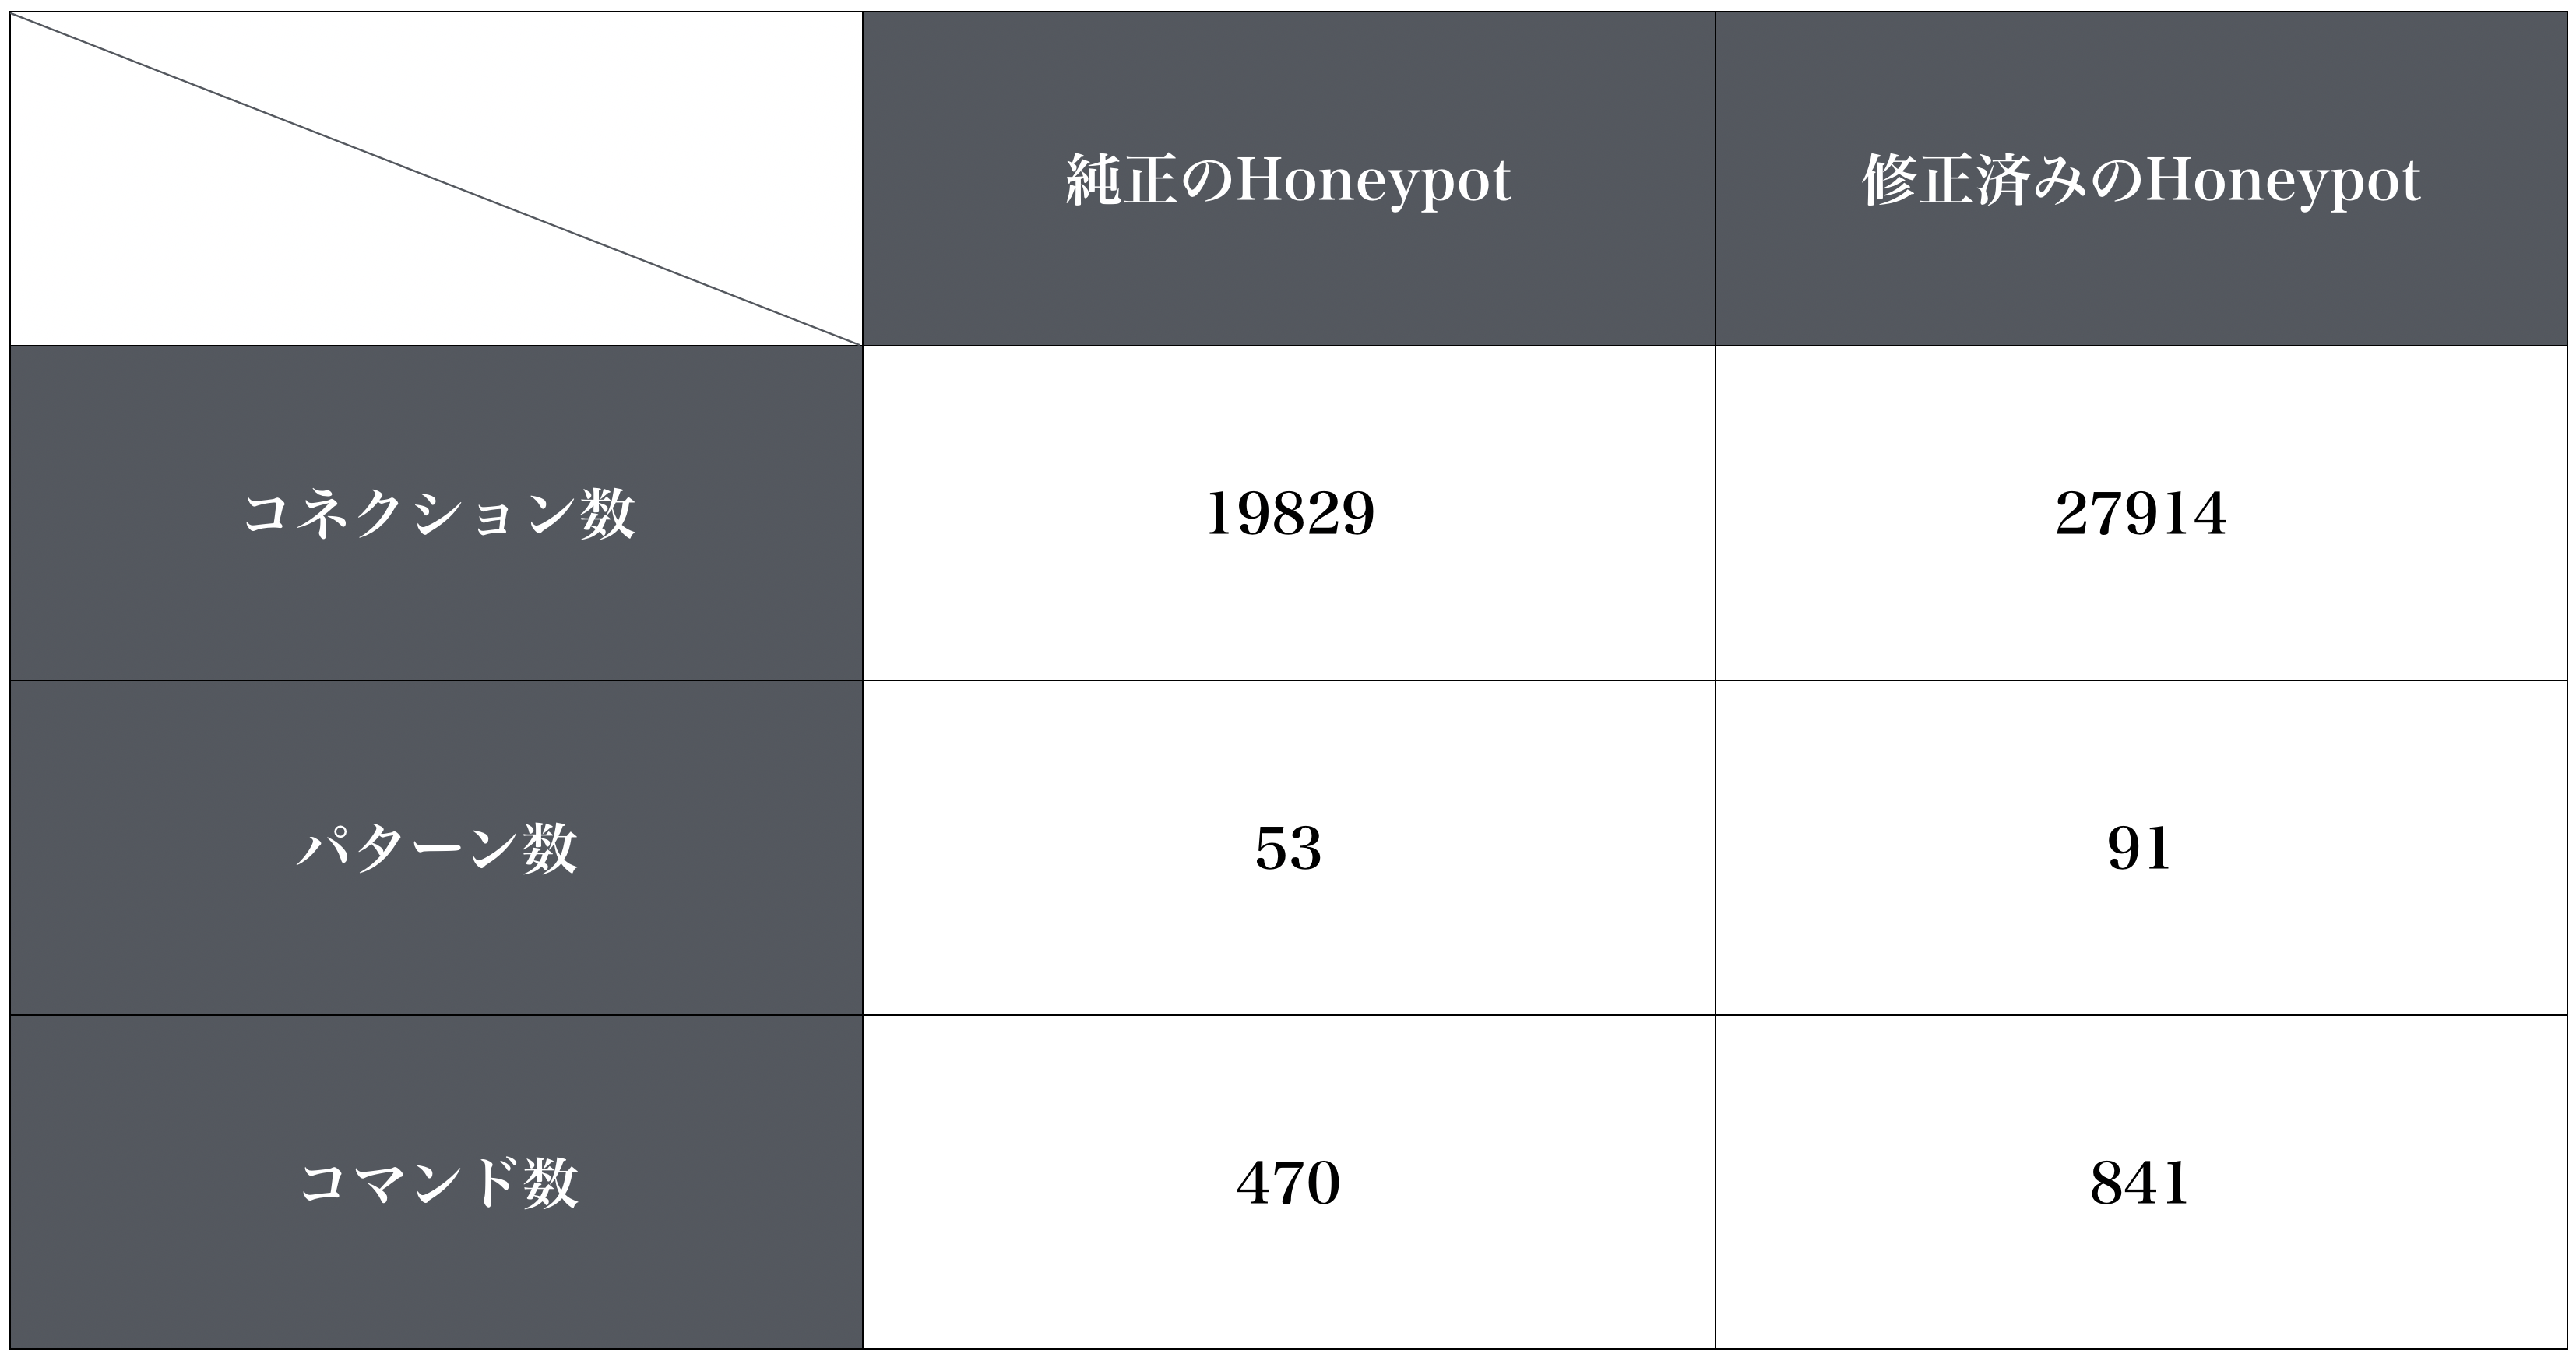
\includegraphics[width=1.0\textwidth]{figures/term.png}
    \caption{収集したSSHの低対話型Honeypotのデータ}
    \label{fig:evo}
\end{figure}

また,モデル化を行い純正のCowrieとCowrieにBusyBoxに含まれるコマンドを実装した修正済みのCowrieのスコアリングを行なった結果を以下の図4に記す.

\begin{figure}[H]
    \centering
    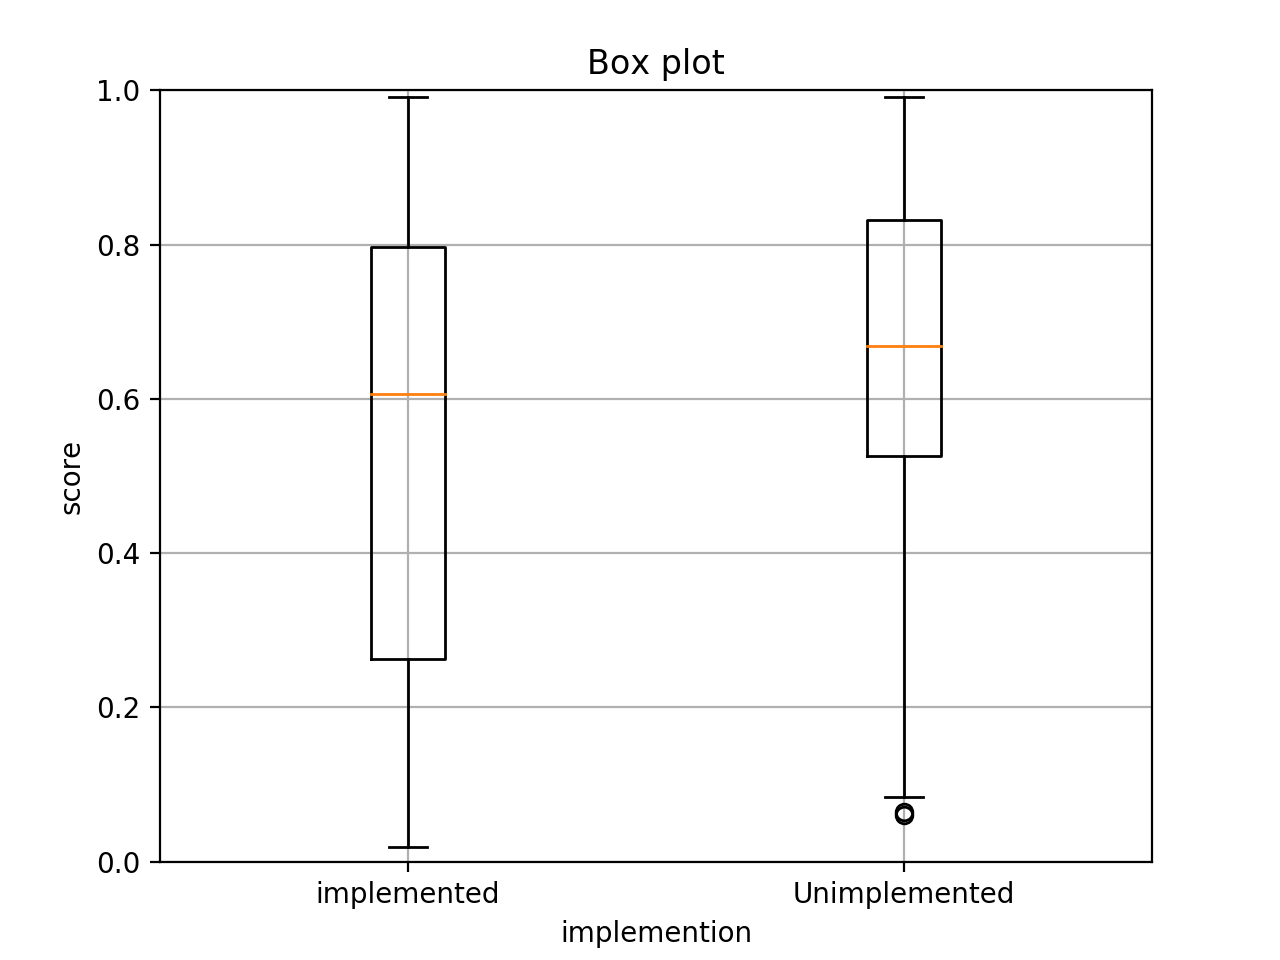
\includegraphics[width=1.0\textwidth]{figures/Figure_1.png}
    \caption{純正のCowrieと修正済みのCowrieのスコアリングによる比較}
    \label{fig:evo}
\end{figure}

本研究の予備実験では,Cowrieに実装されていないコマンドで悪意のある侵入者が使うようなコマンドを実装し,何の追加実装も施していないCowrieで取れた侵入者の実行コマンドログと ,追加実装を施したCowrieの侵入者の実行コマンドログを比較することで,追加実装を施したSSHのCowrieの方がコマンドパターンとして多く収集できることを示した.


%%% Local Variables:
%%% mode: japanese-latex
%%% TeX-master: "../bthesis"
%%% End:
\chapter{本研究の手法}
\label{method}

本章では,~\ref{approach:Hypothesis}節で述べた仮説を検証するために,本研究で行なった手法について概説する.

\section{問題解決の為のアプローチ}
\label{method:approach}
 ~\ref{approach:YotenForProblem}で述べた問題解決のための2つの要件を,本研究の手法として提案する.

 \subsection{コマンドの追加実装}
実際のShellに実装されているコマンドで,SSHの低対話型Honeypotに実装されていないコマンドを実装する.これによってコマンドの追加実装を行なった低対話型Honeypotに侵入した侵入者は,実際のShellと同じような挙動をする低対話型HoneypotをHoneypotであると検知できなくなる.

 \subsection{既実装コマンドの修正}
 SSHの低対話型Honeypotに特有の異常な挙動をする既実装コマンドを修正する.これによって既実装コマンドの修正を行なった低対話型Honeypotに侵入した侵入者は,実際のShellと同じような挙動をする低対話型HoneypotをHoneypotであると検知できなくなる.



%%% Local Variables:
%%% mode: japanese-latex
%%% TeX-master: "../bthesis"
%%% End:
\chapter{実装}
\label{impl}

本章では,低対話型Honeypotと高対話型Honeypotの設置環境についても示し,~\ref{meth:appr}節で述べた手法を用いて純正のHoneypotにどのようなコマンドを実装し,Honeypot特有の異常な挙動を修正したのかを説明する.

\section{実装環境}
本研究で実装するシステムを構成するためのハードウェアおよびソフトウェアについて説明する.表\ref{table:imple}に詳細なバージョンを示す.
\label{impl:env}

% -------------------
\vspace{3mm}
%\newlength{\myheight}
\setlength{\myheight}{10mm}
\begin{table}[h]
 \caption{実装環境}
 \label{table:imple}
 \centering
  \begin{tabular}{|c|c|c|}
   \hline
   ハードウェア/ソフトウェア & 実装環境 & Version(date)  \\
    \hline \hline
     \parbox[c][\myheight][c]{0cm}{} 純正のCowrie  & CentOS5 & 1.4.0  \\
     \hline
     \parbox[c][\myheight][c]{0cm}{} 修正済みのCowrie  & CentOS5 & 1.4.0(self made)  \\
     \hline
     \parbox[c][\myheight][c]{0cm}{} Honeywall  & CentOS5 & 1.4  \\
     \hline
  \end{tabular}
\end{table}
\vspace{7mm}
% --------------------

\subsection{純正のHoneypotで未実装のコマンドの実装}
\label{impl:ImplBusyBox}
本研究において純正のHoneypotはCowrie\cite{cowrie}を使用し,実際のShellには実装されているが,純正のHoneypotで未実装のコマンドについてはBusyBox\cite{busybox}に含まれるコマンドの実装を行なった.~\ref{tech:BusyBox}や~\ref{Cowrie}で紹介した通り,BusyBoxに含まれるコマンドの種類が219ある中で,Cowrieの実装コマンド数は92しか存在しない.この差分をPythonで実装する. \\
またBusyBoxに含まれるコマンドとCowrieの実装コマンドの一覧を表\ref{table:command}に示す. \\
\clearpage
% -------------------

%\geometry
 
\begin{center}
\large{\textbf{実装コマンド一覧}}
\end{center}

BusyBoxに含まれるコマンドとCowrieの実装コマンドの一覧
 
\begin{longtable}{p{100mm}p{100mm}}
  \caption{実装コマンド一覧}
  \label{table:command} \\
  %------ 最初のページの表の最上部 ----
  \hline
  Cowrieの実装コマンド & Busyboxに含まれるコマンド \\ \hline\hline
  \endfirsthead
  %------ 2ページ以降の表の最上部 ----
  \multicolumn{2}{r}{前ページからの続き} \\ \hline
  Cowrieの実装コマンド & Busyboxに含まれるコマンド \\ \hline\hline
  \endhead
  %----- ページの表の最下部 --------
  \hline
  \multicolumn{2}{r}{次ページに続く} \\
  \endfoot
  %----- 最終ページの表の最下部 --------
  \hline
  \multicolumn{2}{r}{以上} \\
  \endlastfoot

     adduser & acpid  \\
     \hline
     alias & adjtimex  \\
     \hline
     apt-get & ar  \\
     \hline
     base64 & arp  \\
     \hline
     bash & arping  \\
     \hline
     busybox & ash  \\
     \hline
     cat & awk  \\
     \hline
     cd & basename  \\
     \hline
     chattr & blockdev  \\
     \hline
     chgrp & brctl  \\
     \hline
     chmod & bunzip2  \\
     \hline
     chown & bzcat  \\
     \hline
     clear & bzip2  \\
     \hline
     cp & cal  \\
     \hline
     curl & cat  \\
     \hline
     date & chgrp  \\
     \hline
     dd & chmod  \\
     \hline
     dget & chown  \\
     \hline
     dir & chpasswd \\
     \hline
     du & chroot \\
     \hline
     echo & chvt \\
     \hline
     egrep & clear \\
     \hline
     env & cmp \\
     \hline
     ethtool & cp \\
     \hline
     exit & cpio \\
     \hline
     export & crond \\
     \hline
     fgrep & crontab \\
     \hline
     free & cttyhack \\
     \hline
     ftpget & cut \\
     \hline
     gcc & date \\
     \hline
     grep & dc \\
     \hline
     halt & dd \\
     \hline
     head & deallocvt \\
     \hline
     help & depmod \\
     \hline
     history & devmem \\
     \hline
     hostname & df \\
     \hline
     id & diff \\
     \hline
     ifconfig & dirname \\
     \hline
     iptables & dmesg \\
     \hline
     jobs & dnsdomainname \\
     \hline
     kill & dos2unix \\
     \hline
     killall & dpkg \\
     \hline
     killall5 & dpkg-deb \\
     \hline
     last & du \\
     \hline
     logout & dumpkmap \\
     \hline
     ls & dumpleases \\
     \hline
     mkdir & echo \\
     \hline
     mv & ed \\
     \hline
     nc & egrep \\
     \hline
     netstat & env \\
     \hline
     nohup & expand \\
     \hline
     passwd & expr \\
     \hline
     perl & FALSE \\
     \hline
     php & fdisk \\
     \hline
     ping & fgrep \\
     \hline
     pkill & find \\
     \hline
     poweroff & fold \\
     \hline
     printf & free \\
     \hline
     ps & freeramdisk \\
     \hline
     pwd & fstrim \\
     \hline
     python & ftpget \\
     \hline
     reboot & ftpput \\
     \hline
     reset & getopt \\
     \hline
     rm & getty \\
     \hline
     rmdir & grep \\
     \hline
     scp & groups \\
     \hline
     service & gunzip \\
     \hline
     set & gzip \\
     \hline
     sh & halt \\
     \hline
     shutdown & head \\
     \hline
     sleep & hexdump \\
     \hline
     ssh & hostid \\
     \hline
     su & hostname \\
     \hline
     sudo & httpd \\
     \hline
     tail & hwclock \\
     \hline
     tar & id \\
     \hline
     tftp & ifconfig \\
     \hline
     touch & ifdown \\
     \hline
     ulimit & ifup \\
     \hline
     umask & init \\
     \hline
     uname & insmod \\
     \hline
     unset & ionice \\
     \hline
     uptime & ip \\
     \hline
     useradd & ipcalc \\
     \hline
     users & kill \\
     \hline
     w & killall \\
     \hline
     wget & klogd \\
     \hline
     which & last \\
     \hline
     who & less \\
     \hline
     whoami & ln \\
     \hline
     yes & loadfont \\
     \hline
     yum & loadkmap \\
     \hline
      & logger \\
     \hline
      & login \\
     \hline
      & logname \\
     \hline
      & logread \\
     \hline
      & losetup \\
     \hline
      & ls \\
     \hline
      & lsmod \\
     \hline
      & lzcat \\
     \hline
      & lzma \\
     \hline
      & lzop \\
     \hline
      & lzopcat \\
     \hline
      & md5sum \\
     \hline
      & mdev \\
     \hline
      & microcom \\
     \hline
      & mkdir \\
     \hline
      & mkfifo \\
     \hline
      & mknod \\
     \hline
      & mkswap \\
     \hline
      & mktemp \\
     \hline
      & modinfo \\
     \hline
      & modprobe \\
     \hline
      & more \\
     \hline
      & mount \\
     \hline
      & mt \\
     \hline
      & mv \\
     \hline
      & nameif \\
     \hline
      & nc \\
     \hline
      & netstat \\
     \hline
      & nslookup \\
     \hline
      & od \\
     \hline
      & openvt \\
     \hline
      & passwd \\
     \hline
      & patch \\
     \hline
      & pidof \\
     \hline
      & ping \\
     \hline
      & ping6 \\
     \hline
      & pivot\_root \\
     \hline
      & poweroff \\
     \hline
      & printf \\
     \hline
      & ps \\
     \hline
      & pwd \\
     \hline
      & rdate \\
     \hline
      & readlink \\
     \hline
      & realpath \\
     \hline
      & reboot \\
     \hline
      & renice \\
     \hline
      & reset \\
     \hline
      & rev \\
     \hline
      & rm \\
     \hline
      & rmdir \\
     \hline
      & rmmod \\
     \hline
      & route \\
     \hline
      & rpm \\
     \hline
      & rpm2cpio \\
     \hline
      & run-parts \\
     \hline
      & sed \\
     \hline
      & seq \\
     \hline
      & setkeycodes \\
     \hline
      & setsid \\
     \hline
      & sh \\
     \hline
      & sha1sum \\
     \hline
      & sha256sum \\
     \hline
      & sha512sum \\
     \hline
      & sleep \\
     \hline
      & sort \\
     \hline
      & start-stop-daemon \\
     \hline
      & stat \\
     \hline
      & static-sh \\
     \hline
      & strings \\
     \hline
      & stty \\
     \hline
      & su \\
     \hline
      & sulogin \\
     \hline
      & swapoff \\
     \hline
      & swapon \\
     \hline
      & switch\_root \\
     \hline
      & sync \\
     \hline
      & sysctl \\
     \hline
      & syslogd \\
     \hline
      & tac \\
     \hline
      & tail \\
     \hline
      & tar \\
     \hline
      & taskset \\
     \hline
      & tee \\
     \hline
      & telnet \\
     \hline
      & telnetd \\
     \hline
      & test \\
     \hline
      & tftp \\
     \hline
      & time \\
     \hline
      & timeout \\
     \hline
      & top \\
     \hline
      & touch \\
     \hline
      & tr \\
     \hline
      & traceroute \\
     \hline
      & traceroute6 \\
     \hline
      & TRUE \\
     \hline
      & tty \\
     \hline
      & tunctl \\
     \hline
      & udhcpc \\
     \hline
      & udhcpd \\
     \hline
      & umount \\
     \hline
      & uname \\
     \hline
      & uncompress \\
     \hline
      & unexpand \\
     \hline
      & uniq \\
     \hline
      & unix2dos \\
     \hline
      & unlzma \\
     \hline
      & unlzop \\
     \hline
      & unxz \\
     \hline
      & unzip \\
     \hline
      & uptime \\
     \hline
      & usleep \\
     \hline
      & uudecode \\
     \hline
      & uuencode \\
     \hline
      & vconfig \\
     \hline
      & vi \\
     \hline
      & watch \\
     \hline
      & watchdog \\
     \hline
      & wc \\
     \hline
      & wget \\
     \hline
      & which \\
     \hline
      & who \\
     \hline
      & whoami \\
     \hline
      & xargs \\
     \hline
      & xz \\
     \hline
      & xzcat \\
     \hline
      & yes \\
     \hline
      & zcat \\
     \hline
\end{longtable}
%\vspace{3mm}
%\setlength{\myheight}{10mm}
%\begin{table}[h]
% \caption{実装コマンド一覧}
% \label{table:command}
% \centering
%  \begin{tabular}{|c|c|}
%   \hline
%   Busyboxに含まれるコマンド & Cowrieの実装コマンド  \\
%    \hline \hline
%  \end{tabular}
%\end{table}
%\vspace{7mm}
% --------------------

%%% Local Variables:
%%% mode: japanese-latex
%%% TeX-master: "../bthesis"
%%% End:

\chapter{評価と考察}
\label{eval}

本章では,予備実験と\ref{impl}章で実装した本研究での提案手法の評価とその考察を述べる.

\section{予備実験}
\label{eval:first}

%\subsection{概要}
%\label{eval:abst}
SSHの低対話型HoneypotであるCowrieはコマンドの実装数が少なく,Cowrie特有の異常な挙動が多い.そのため,侵入者にHoneypotであると検知されることで,本来実際のOSへの攻撃であれば取れるはずであった侵入ログが取れない問題がある.また,収集ログを分析する際に,これまで用いられてきた"危険なコマンド"としてインデックスを作り,それらを危険なコマンドとしてパターンマッチングする手法では,今後出現してくる様々なコマンドパターンなどに対応できない.\\
予備実験では,Cowrieはコマンドの実装数が少なく,Cowrie特有の異常な挙動が多いため,コマンドの追加実装を行い,Cowrie特有の異常な挙動を修正した.実装を施していない純正のCowrieとCowrieにBusyBoxに含まれるコマンドを実装した修正済みのCowrieの両方でコマンドログの収集を行い,比較することで,収集ログのパターンの変化を観測できるのではないかと考えた.評価として収集した二つのログをSkip-gramモデルを用いてスコアリングし,どちらがより多くのコマンドログのパターンを収集できているのかを検証した.\\
その結果,より多くのコマンドパターンを取れたのがCowrieにBusyBoxに含まれるコマンドを実装した修正済みのCowrieであるということが明らかとなった.

\subsection{予備実験の手法}
\label{eval:appr}
実装を施していない純正のCowrieに対して,これには実装されていないがShellには実装されているコマンドを実装したものを設置し,ログを収集した.

\subsection{侵入ログの収集環境}
\label{eval:apprenv}


\subsection{実装}
\label{eval:impl}
純正のCowrieにBusyBoxに含まれるコマンドを実装し,またHoneypot特有の異常な挙動を修正した.ここでの実装を紹介する.

\subsection{評価}
\label{eval:eval}
実装を施していない純正のCowrieとCowrieにBusyBoxに含まれるコマンドを実装した修正済みのCowrieの両方で侵入ログの収集を行い,Word2vecのSkip-Gram Modelにより次のコマンドの予測,スコアリングを行い比較を行うことで,差異を評価した.スコアリングでは,あるコマンドが実行された時に次のコマンドの出やすさを予測したため,次に実行されるコマンドがスコアとして高い数値を出せばそのコマンドパターンがパターンとして存在しやすいものであることを示す.予備実験の評価に関しては第7章の評価で一部説明している.
本研究の評価と評価手法の違いは,モデル化を純正のHoneypotにBusyBoxに含まれるコマンドを実装したものしか行っていないため,実際のOSに近いログが取れたことが証明できておらず,比較する対象が少なかった.

\subsection{結果}
\label{eval:conc}
SSHの低対話型Honeypotの稼働期間は12/10から2/1(54日間)で,収集できたものとしてコネクション数,パターン数,コマンド数を以下の表\ref{table:kenchi}に記す.

% -------------------
\vspace{3mm}
\newlength{\myheighta}
\setlength{\myheighta}{10mm}
\begin{table}[h]
 \caption{予備実験の結果}
 \label{table:kenchi}
 \centering
  \begin{tabular}{|c||c|c|}
   \hline
   \parbox[c][\myheighta][c]{0cm}{} 検知したもの & 純正のHoneypot & 修正済みのHoneypot \\
   \hline \hline 
     \parbox[c][\myheighta][c]{0cm}{} コネクション数  & 19829 & 27914 \\
     \hline
     \parbox[c][\myheighta][c]{0cm}{} パターン数  & 53 & 91 \\
     \hline
     \parbox[c][\myheighta][c]{0cm}{} コマンド数  & 470 & 841 \\
     \hline
  \end{tabular}
\end{table}
\vspace{5mm}
% -------------------

%\begin{figure}[htbp]
%    \centering
%    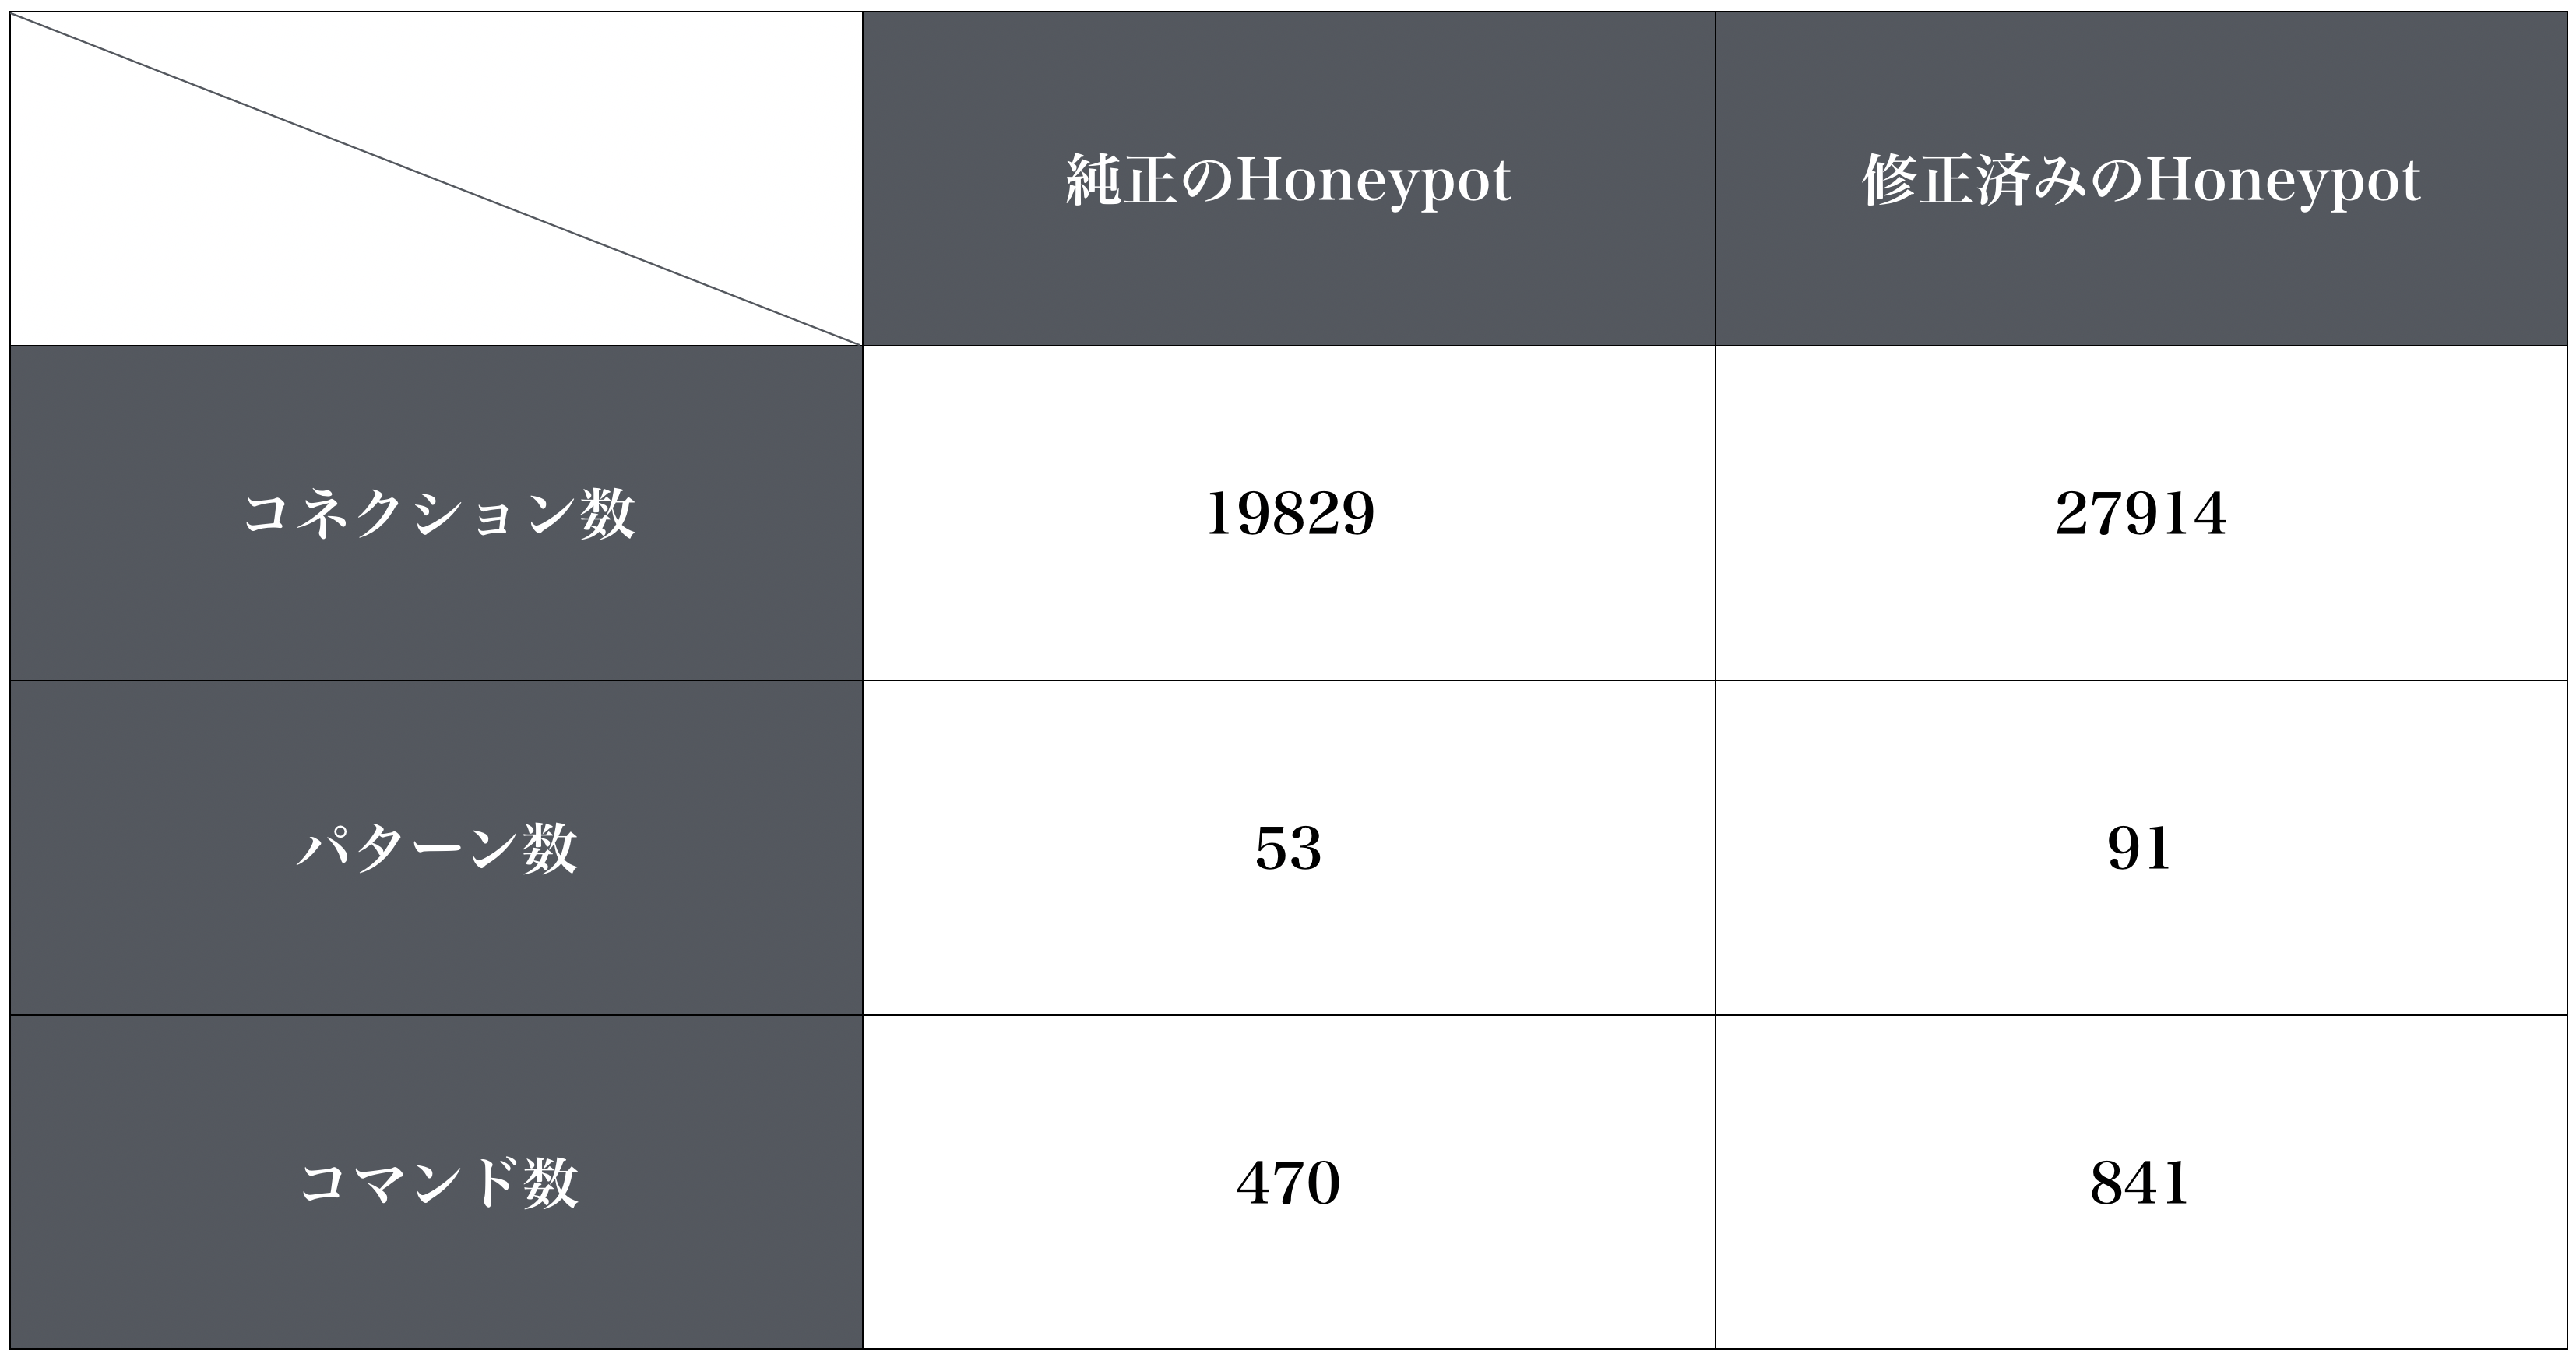
\includegraphics[width=1.0\textwidth]{figures/term.png}
%    \caption{収集したSSHの低対話型Honeypotのデータ}
%    \label{fig:honeypotdata}
%s\end{figure}

また,モデル化を行い純正のCowrieとCowrieにBusyBoxに含まれるコマンドを実装した修正済みのCowrieのスコアリングを行なった結果を以下の図\ref{fig:cowriecompare}に記す.横軸はコマンド拡張を行なったHoneypotか素のHoneypotであるかを示している.縦軸は予備実験の評価手法によって算出されたコマンドの表れやすさを数値化したものであり,数値が高くなればのコマンドパターンがパターンとして存在しやすいものであることを示している.予備実験ではコマンドの拡張実装をしたものの方がコマンドパターンとして存在しにくいものを観測できたという結果になった.

\begin{figure}[htbp]
    \centering
    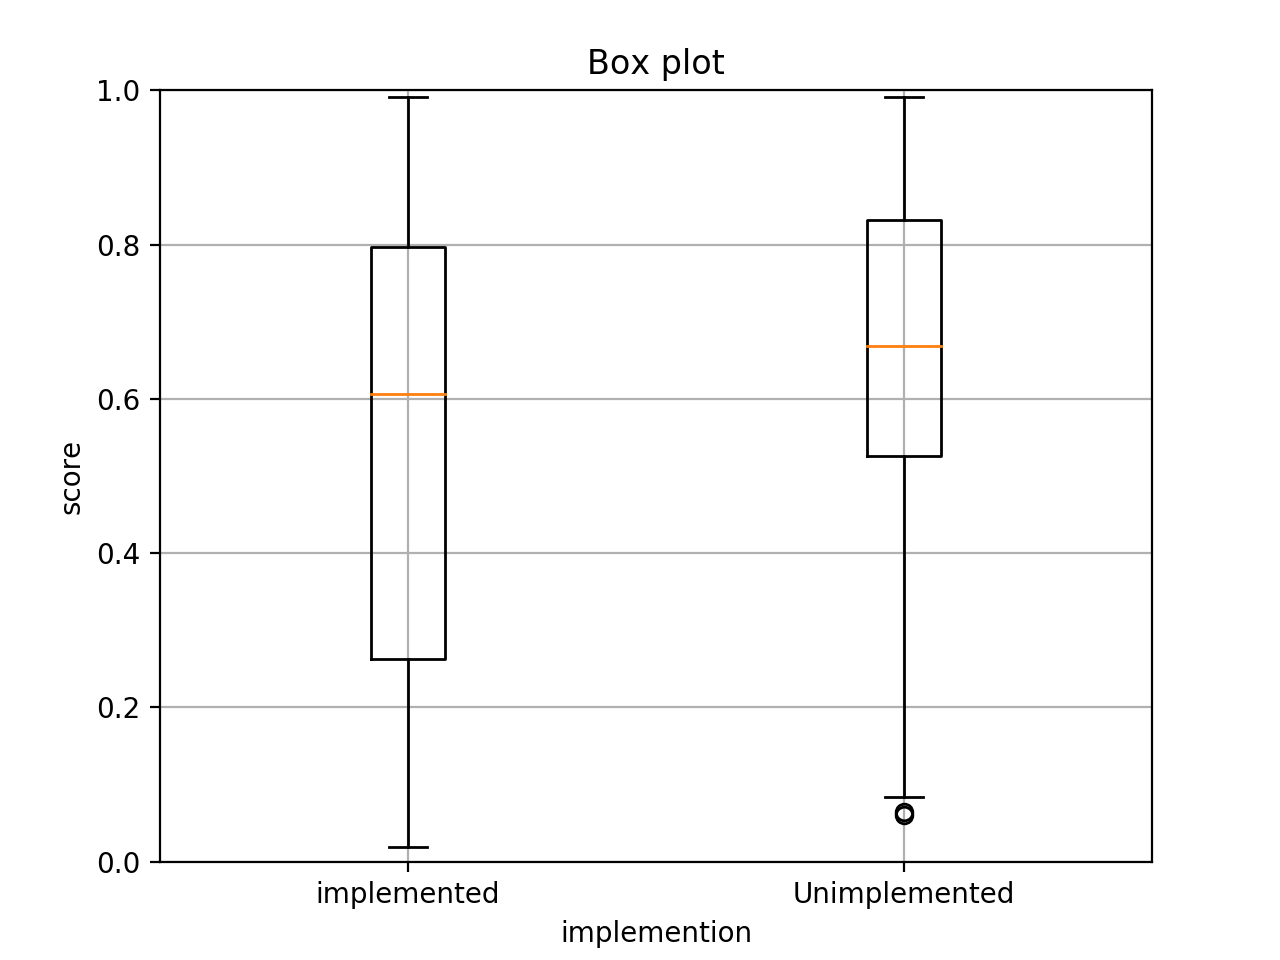
\includegraphics[width=1.0\textwidth]{figures/Figure_1.png}
    \caption{純正のCowrieと修正済みのCowrieのスコアリングによる比較}
    \label{fig:cowriecompare}
\end{figure}

本研究の予備実験では,Cowrieに実装されていないコマンドで悪意のある侵入者が使うようなコマンドを実装し,何の追加実装も施していないCowrieで取れた侵入者の実行コマンドログと ,追加実装を施したCowrieの侵入者の実行コマンドログを比較することで,追加実装を施したSSHのCowrieの方がコマンドパターンとして多く収集できることを示した.


\section{評価手法}
\label{eval:eval}

本研究の仮説の検証手法としての評価として,~\ref{appr:YotenForProblem}節で述べた要件に対して評価を行う.\\
予備実験では,素の低対話型Honeypotよりも,コマンドを拡張したHoneypotの方がコマンドパターンが多く収集できることを示した.本研究では拡張したHoneypotで収集したコマンドログが,どれほど一般的なUNIXユーザーの実行するコマンドから離れたのかを評価した.\\
本研究では,以下の三種類のHoneypotを設置する.\\
1. 広く利用されているSSHの低対話型Honeypot\\
2. 実際のShellには実装されているが,1.のHoneypotで未実装のコマンドを実装したHoneypot\\
3. 広く利用されている高対話型Honeypot\\

これ以降,1.の広く利用されているSSHの低対話型Honeypotのことを”純正の低対話型Honeypot” , 2.の実際のShellには実装されているが,1.のHoneypotで未実装のコマンドを実装したHoneypotのことを"修正済みの低対話型Honeypot" , 3.の広く利用されている高対話型Honeypotのことを"高対話型Honeypot"と呼ぶこととする.\\

%以上3つの純正のHoneypot,修正済みのHoneypot,高対話型Honneypotのそれぞれで侵入ログを収集する.\\

また予備実験では,純正のHoneypotに実装されていないコマンドで悪意のある侵入者が使うようなコマンドを実装し,純正のHoneypotで取れた侵入者の実行コマンドログと,修正済みのHoneypotの侵入者の実行コマンドログを比較することで,修正済みのHoneypotの方がコマンドパターンとして多く収集できることを示した.予備実験における収集ログの比較の概念図を図\ref{fig:yobigainen}に示す.

\begin{figure}[htbp]
    \centering
    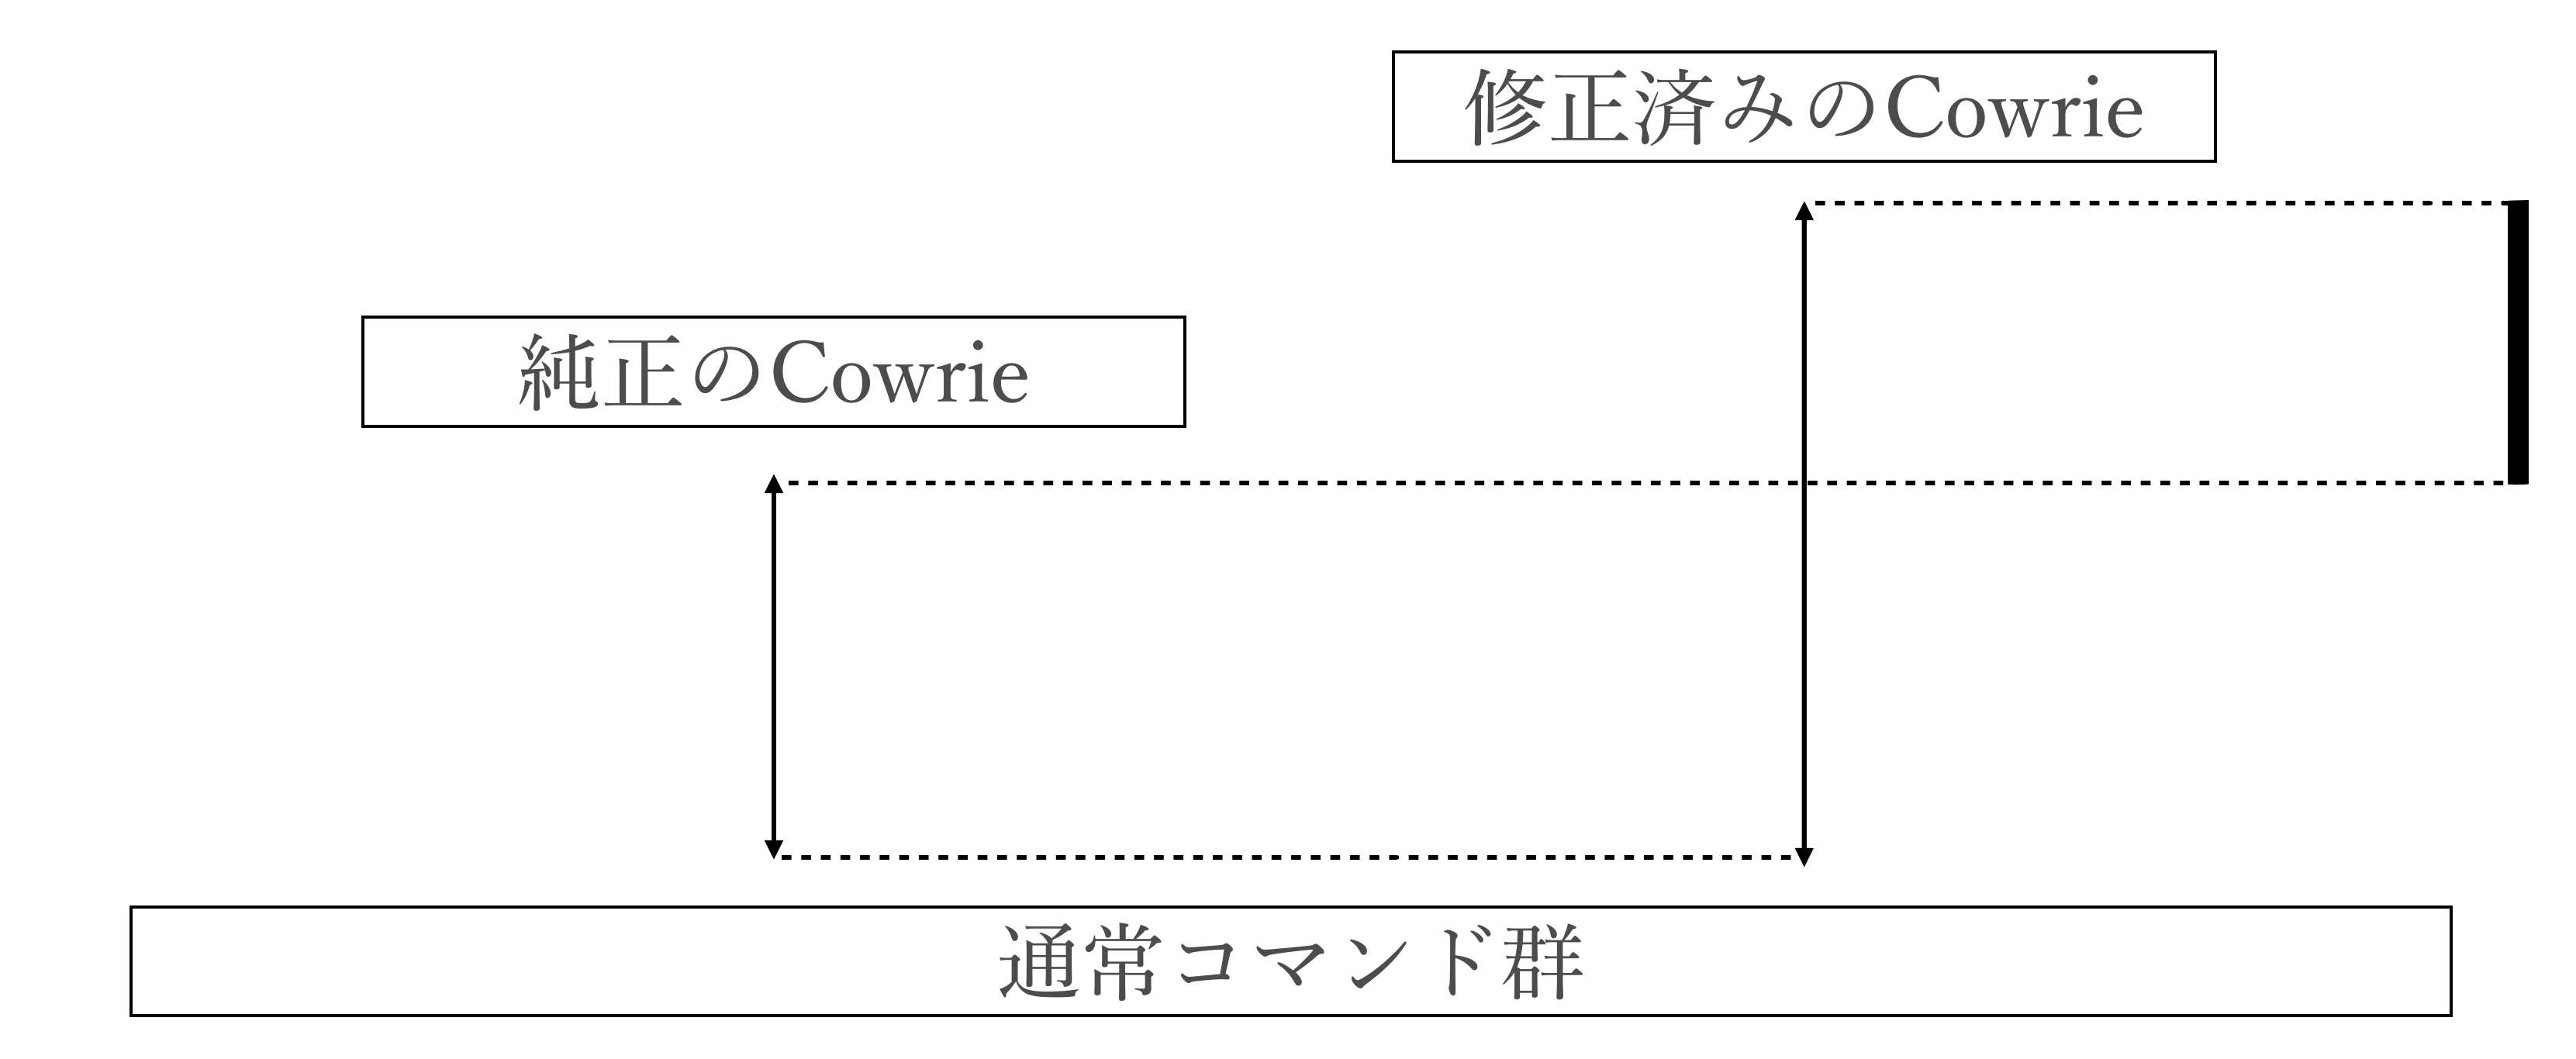
\includegraphics[width=1.0\textwidth]{figures/termhyoka.png}
    \caption{予備実験の評価の概念図}
    \label{fig:yobigainen}
\end{figure}

この予備実験では評価として何の追加実装も施していないSSHの低対話型Honeypotで取れた侵入者の実行コマンドログと追加実装を施したSSHの低対話型Honeypotの侵入者の実行コマンドログとを比較したのに対して,本件研究の評価手法では,純正のHoneypotで取れた侵入者の実行コマンドログと修正済みのHoneypotの侵入者の実行コマンドログと高対話型Honeypotの侵入者の実行コマンドログを比較することで,修正済みのHoneypotの侵入者の実行コマンドログが一般的なUNIXユーザーの実行するコマンドから離れたのかを評価した.%研究における収集ログの比較の概念図を図\ref{fig:gainen}に示す.

%\begin{figure}[htbp]
%    \centering
%    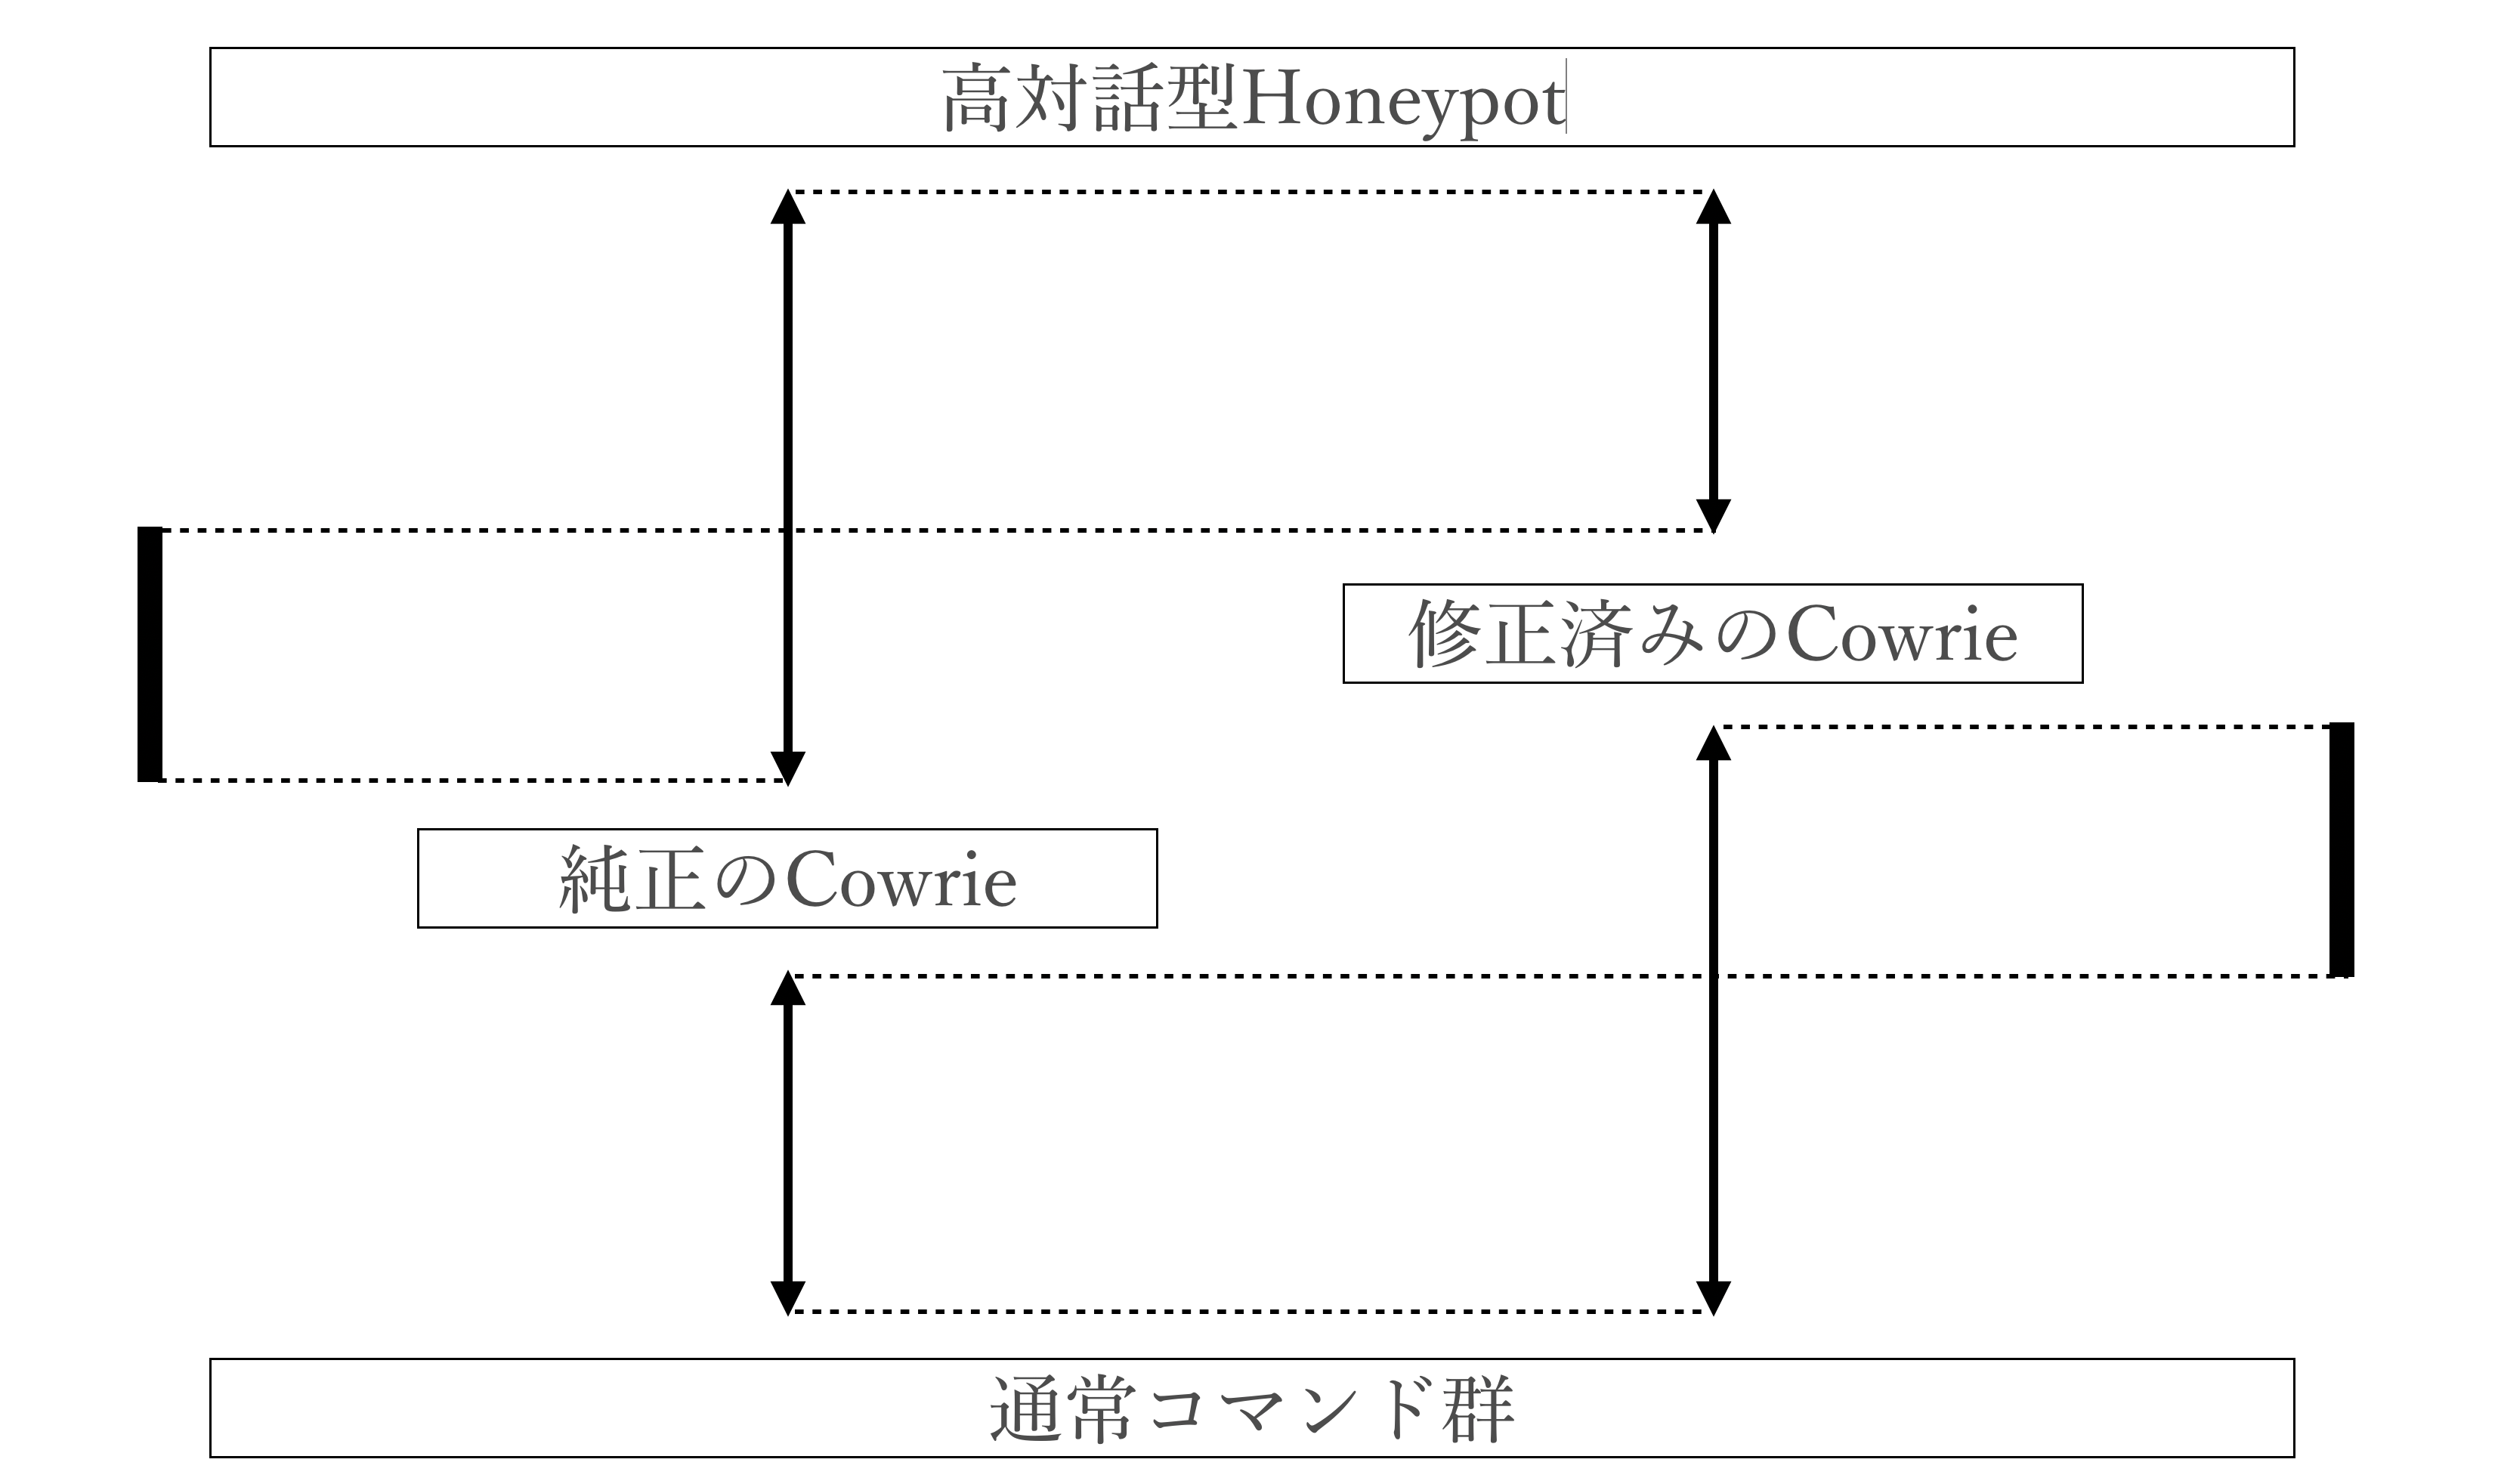
\includegraphics[width=1.0\textwidth]{figures/sotuhyoka.png}
%    \caption{本研究の評価の概念図}
%    \label{fig:gainen}
%\end{figure}



\subsection{コマンドログのスコアリング手法の実装の提案}
\label{eval:implsuge}
コマンドログの比較を行う手法は多く存在する.例えば評価基準として,あるコマンドが実行された時に,そのコマンドは危険であるとしたブラックリストを作成するパターンマッチングの手法がある.また,攻撃であるとされたコマンドを~\ref{tech:Markov}で説明したマルコフモデルで学習させることで,攻撃性を表現する手法がある.
しかしパターンマッチングであれば静的解析であるので未知の攻撃に対応ができず,マルコフモデルであれば現在の状態だけに依存して次の状態への推移確率が決まるので,未知の特徴量を無視してしまうので,いずれも未知の攻撃に対応できない.
しかし,~\ref{tech:NLP}で説明した意味解析をコマンドログに導入することで,コマンド名が別でも同じような内容のコマンドを実行しようとした時に,それが同じような内容であることを検知できる自然言語処理における意味解析のニューラルネットワークのモデルを評価基準とすることで未知の攻撃にも対応できる.
そのため,本研究では自然言語処理における意味解析のニューラルネットワークのモデルを評価基準とした.

\subsection{機械学習を用いたコマンドログのスコアリング}
\label{eval:impl}
本研究では,評価基準となる,自然言語処理における意味解析のニューラルネットワークのモデルとしてWord2vecのskip-gramモデルを採用した.
純正の低対話型Honeypotで収集した侵入ログでskip-gramモデルの隠れ層の重みを学習させ(これをモデル1
とする),同様にして高対話型Honeypotで収集した侵入ログもskip-gramモデルの隠れ層の重みを学習させる(これをモデル2とする).次に修正済みのHoneypotで収集したログをセッション開始からセッション終了までに打たれたコマンドごとに(以降これを1セッションごとと呼ぶ)モデル1とモデル2のそれぞれに入力していき,出力された数値aを活性化関数としてソフトマックス関数をかけることで,0≦a≦1の範囲を取るようにし確率的な数値として出力することでスコアリングを行う.このため入力に対して多数存在する出力を全てを合計すると1になる.
純正の低対話型Honeypotや高対話型Honeypotの収集ログをモデル化する際、入力層として収集ログのコマンドの入力に対してそのコマンドの周辺のコマンドを出力として与えることでこれを学習させる.\\
例えば3つのコマンドが打たれたとしたとしたものを以下のプログラム\ref{lst:exam}に示す.

\vspace{5mm}
%\lstnewenvironment{mylisting}[1][]
%    {\lstset{
%        frame=single,
%        basicstyle=\ttfamily,
%        numbers=left,
%        numbersep=10pt,
%        tabsize=2,
%        extendedchars=true,
%        xleftmargin=17pt,
%        framexleftmargin=17pt,
%        #1
%    }
%}{}

\begin{mylisting}[label=exam,language=sh,caption=3つの実行コマンドの例]
 $ uname
 $ free
 $ ps x
 $
\end{mylisting}
\vspace{5mm}

モデルを構築する際には"free"コマンドを入力にした時に,出力として"uname"コマンド"ps"コマンドを用意しておくことで,freeが入力として与えられた時に他2つの出力される周辺のコマンドが出力する確率が高くなるようにする.また,実装としては周辺語をどこまで広げるのかはパラメータとしてwindow sizeで与えることができ,上記の例の周辺語は"1"であり,window sizeを"2"にすればモデル化する際に出力層に与えられる数は4つとなる.
以下の図\ref{fig:hyoukaflow}にモデル化のフローを示す.\\

\vspace{10mm}
\begin{figure}[htbp]
    \centering
    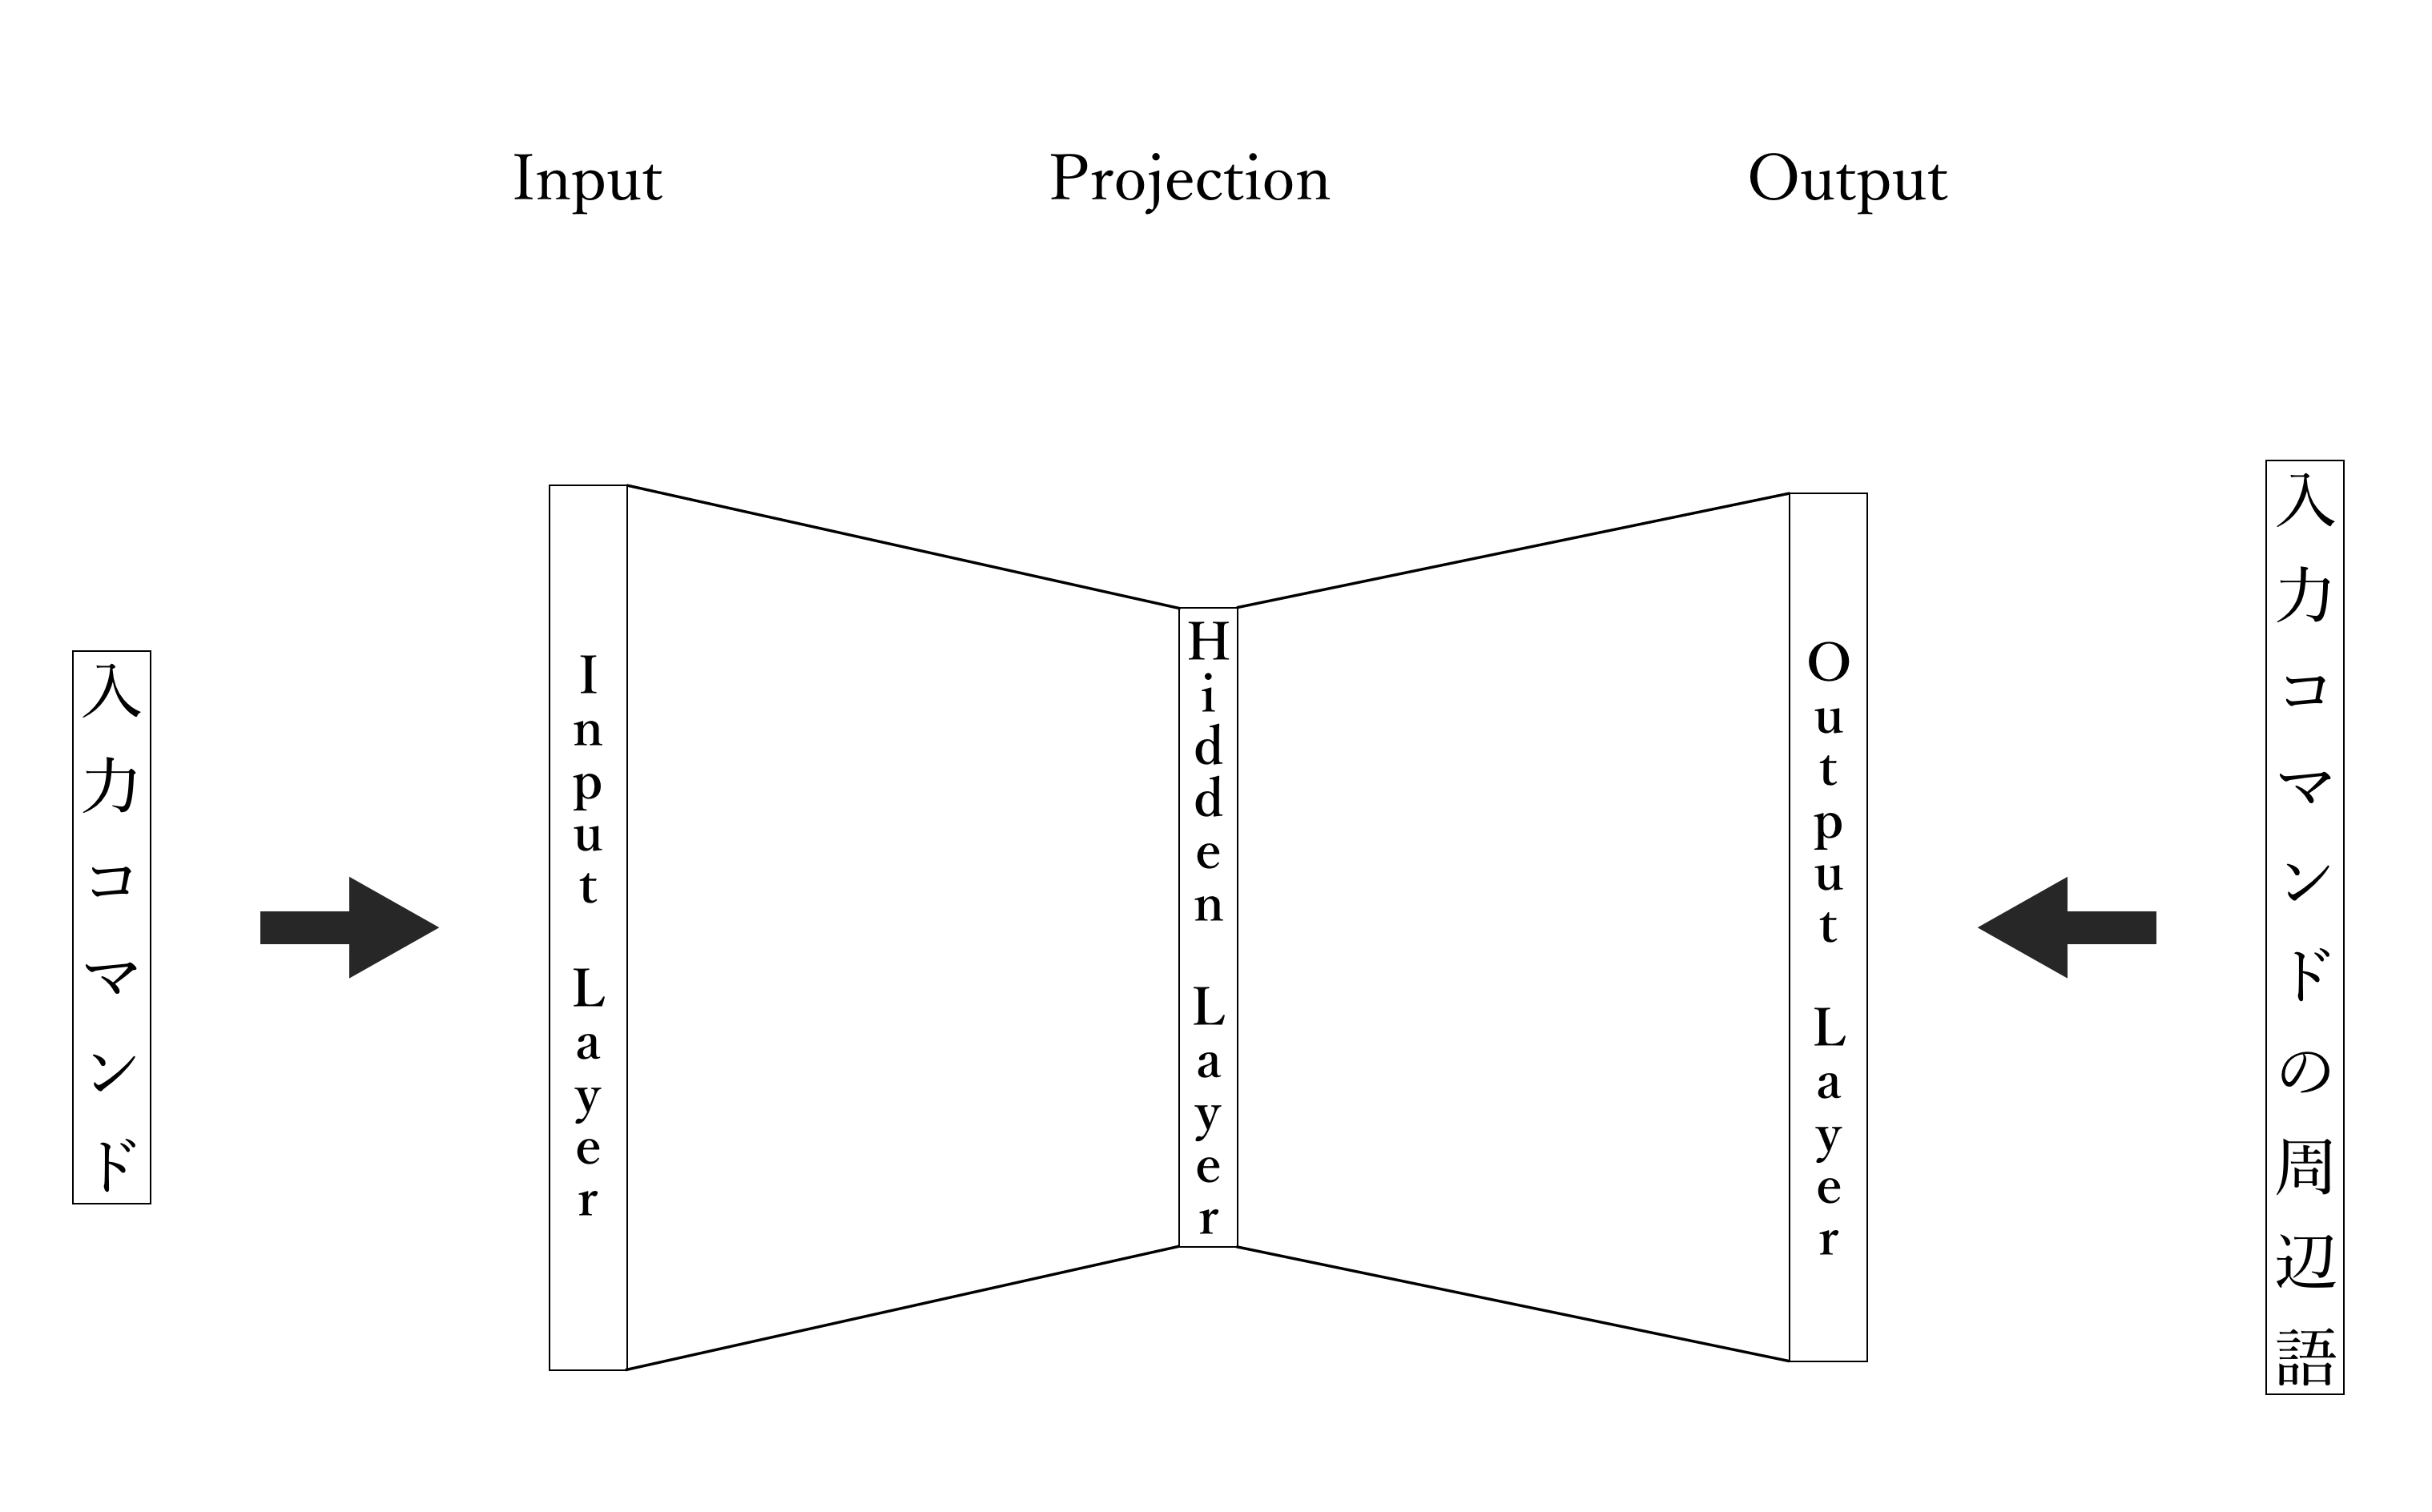
\includegraphics[width=1.0\textwidth]{figures/model.png}
    \caption{評価のフロー\cite{word2vecpaper}\cite{word2vecpaper2}}
    \label{fig:hyoukaflow}
\end{figure}
\vspace{10mm}
\clearpage

また,このようにして純正の低対話型Honeypotの収集ログと高対話型Honeypotの収集ログに対して各々のモデルを構築する.次にこのモデルに対して,修正済みのHoneypotで収集したログを入力して,確率的にスコアリングしていくことで数値を出力する.\\

以下にこのモデルを使用した時の入力から出力のフローを図\ref{fig:syuturyokuflow}を示す.\\

\begin{figure}[htbp]
    \centering
    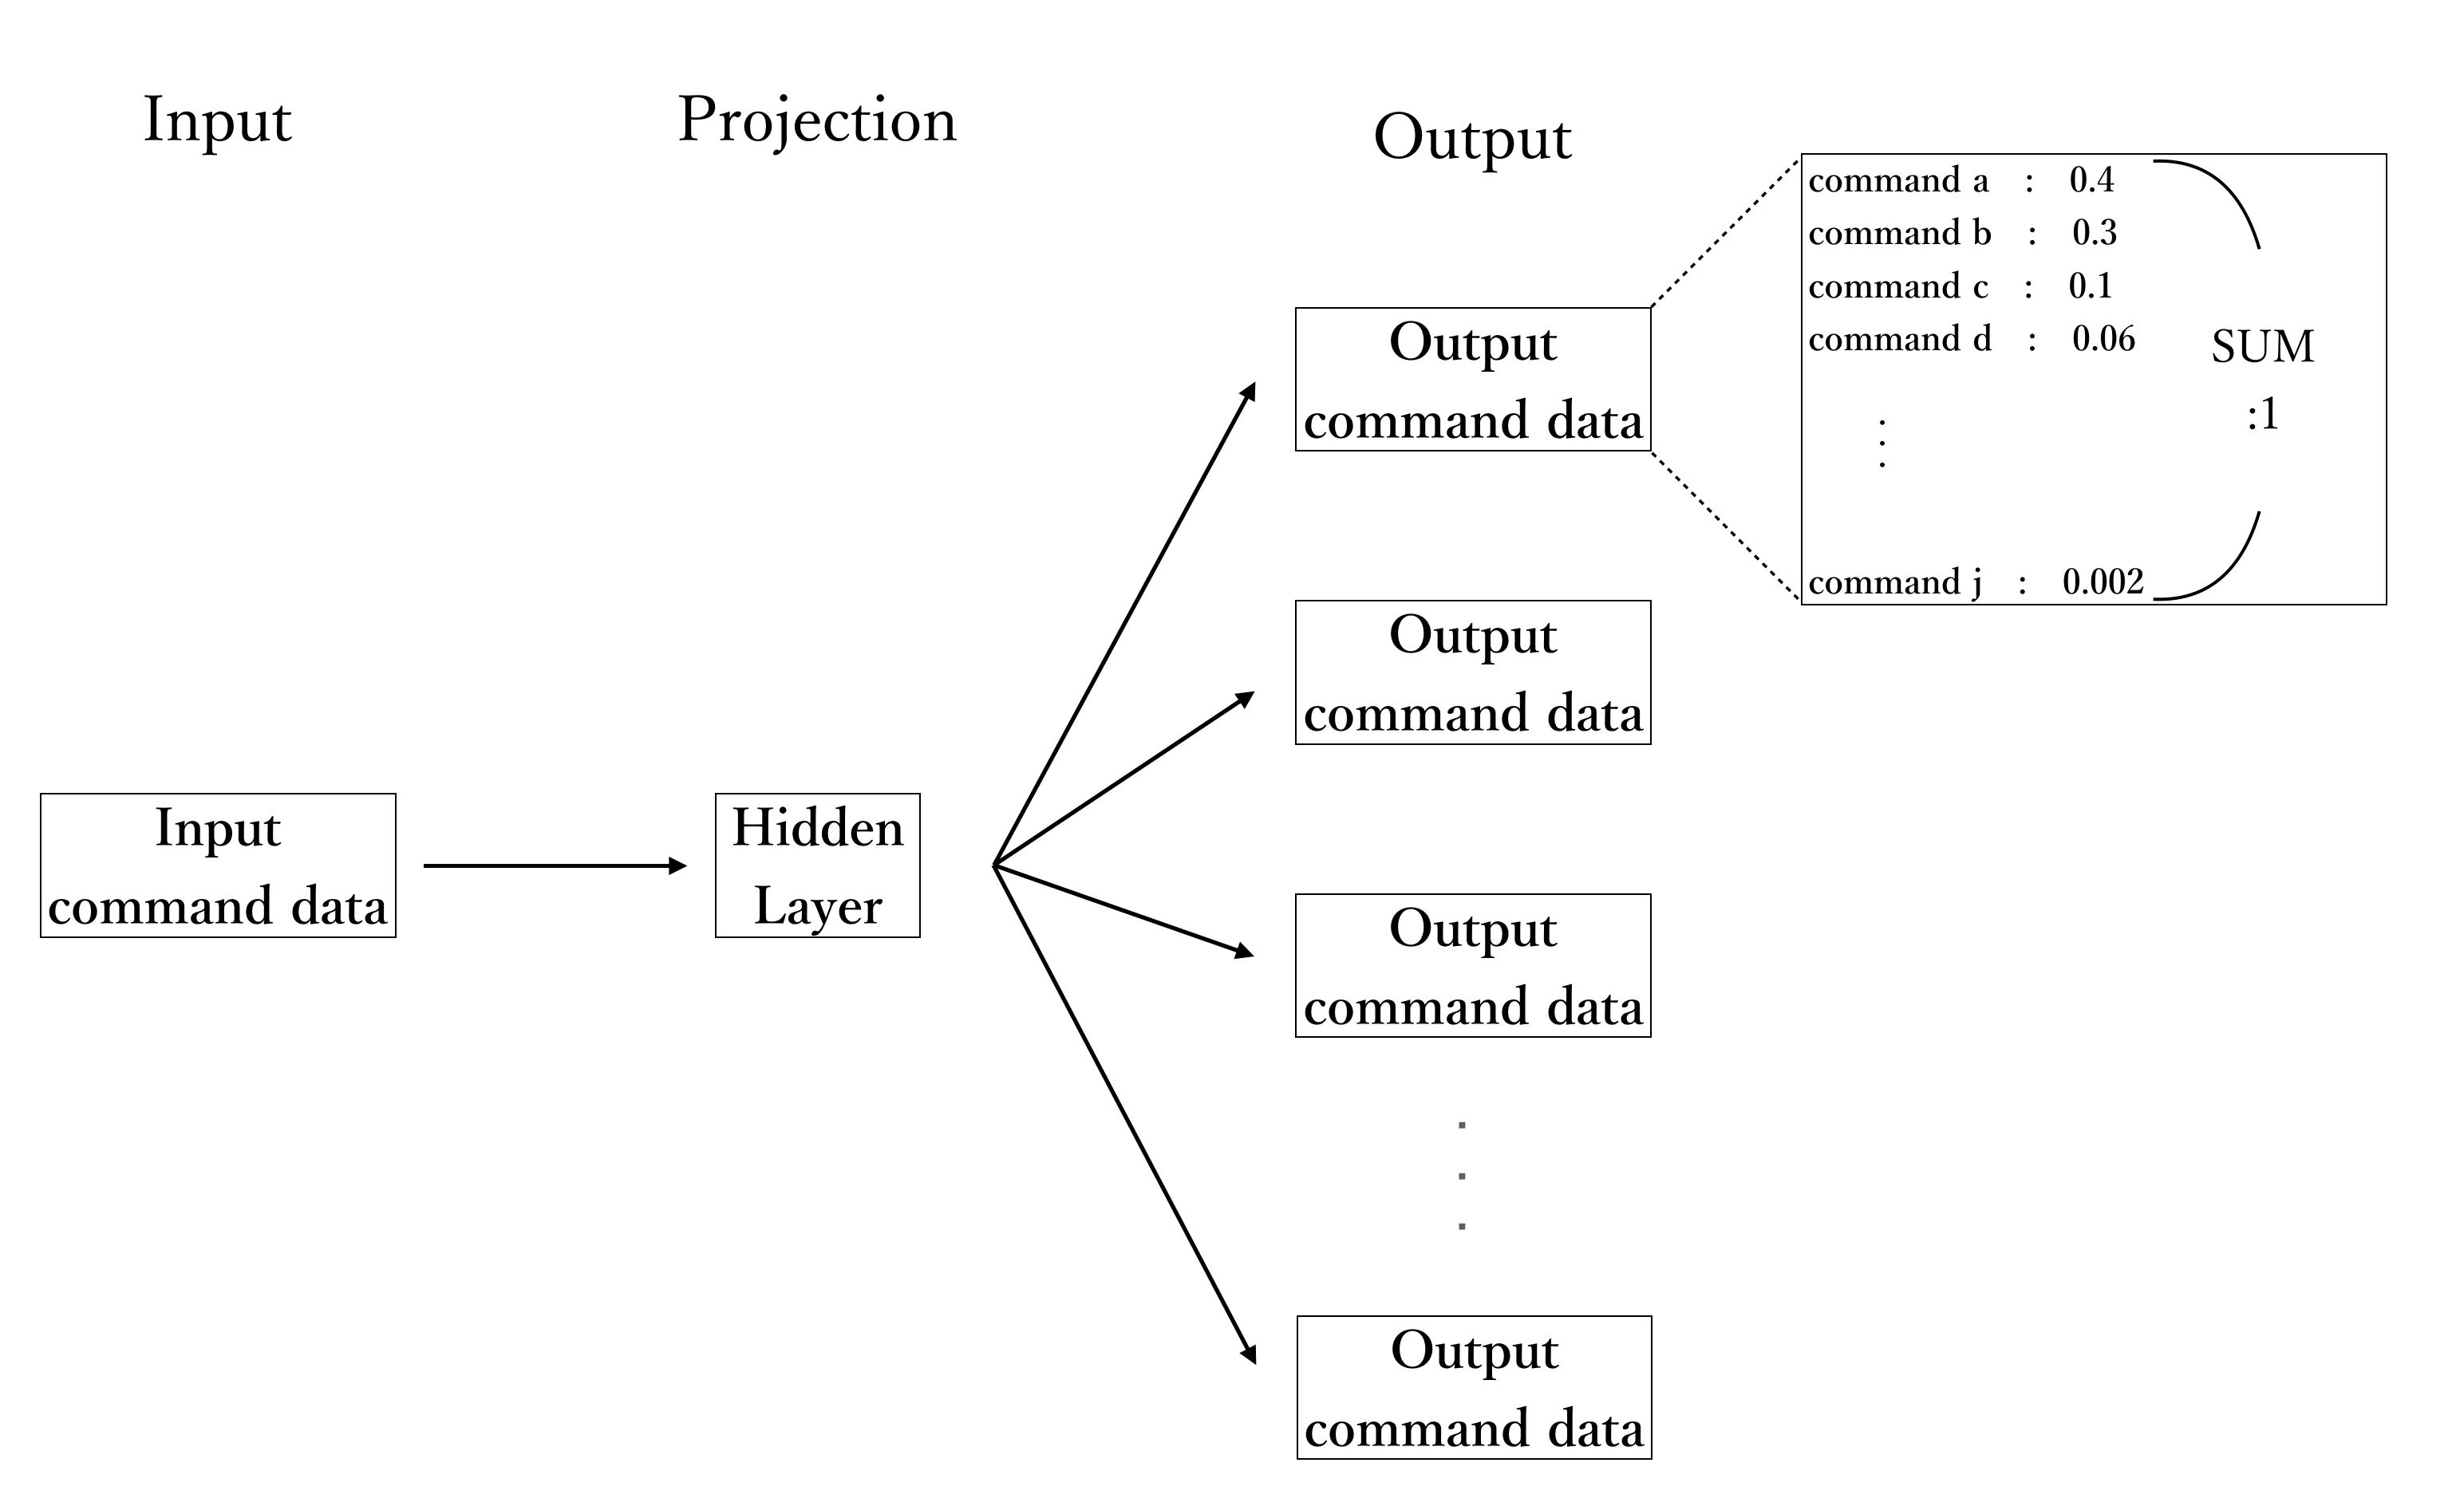
\includegraphics[width=1.0\textwidth]{figures/evalflow.png}
    \caption{評価のフロー\cite{word2vecpaper}\cite{word2vecpaper2}}
    \label{fig:syuturyokuflow}
\end{figure}

このようにして出力された数値を1セッションごとに平均化し,また全てのセッションにおいてもセッションごとに平均化し,全てのセッションの平均化を行うことで,純正の低対話型Honeypotの収集ログと高対話型Honeypotの収集ログとの各々で構築したモデルごとに平均値を算出する.


\subsubsection{コマンド群データのベクトル表現}
\label{eval:CommandVector}

\subsubsection{SSHの低対話型Honeypotの攻撃ログの比較}
\label{eval:CompareLog}


\section{考察}
\label{eval:implkosatu}

%%% Local Variables:
%%% mode: japanese-latex
%%% TeX-master: "./thesis"
%%% End:

\chapter{関連研究}
 \label{rela}

\section{関連研究}
本章では,SSHのHoneypotと時系列データの処理に関連する先行研究について紹介する.
\subsection{SSHのHoneypot}
%\subsubsection{低対話型Honeypot}
%\subsubsubsection{kiipo}
%\subsubsubsection{cowrie}
%\subsubsection{高対話型Honeypot}
%\subsubsubsection{honeynet}
% \makeendnotes  %make notes at the last of this chapter // if you do not  want use endnotes style, please comment out this.
\subsection{自然言語処理における意味解析}
~\ref{tech:NLP}で述べたように,自然言語処理とは人間が日常的に使っている自然言語をコンピュータに処理させる一連の技術である.現在,意味解析において大きくシソーラス解析とベクトル空間分析の2つが手法として多く,本研究ではこのうちベクトル空間分析を使用した.そのため関連研究ではベクトル空間解析について述べる.
\subsubsection{ベクトル空間解析}
~\ref{tech:Vector}で述べたように,自然言語処理の意味解析の手法の一つにベクトル空間解析というものがある.本研究で取得したHoneypotのデータを用いて,ベクトル空間解析の他の手法でもでも評価を試みた.
\subsubsubsection{ベクトル空間モデル}
~\ref{tech:voctorkukan}で述べたように,ベクトル空間解析にはベクトル空間モデルというものが存在する.~\ref{tech:tfidf}で述べたTF-IDFを用いて,同一文章内での単語の出現頻度と,様々な文章におけるある単語の逆文書頻度の2つを重みとし,文章を多次元マトリクスで表現する.文章同士の距離をなす角$ \theta $の,$ 0^\circ \leqq \theta \leqq 90^\circ $における$ \cos \theta $の値の大きさによって文章の類似度を算出する.多次元マトリクスにおける2つの文章のベクトルの方向は文章の特徴であるので,$ 0^\circ \leqq \theta \leqq 90^\circ $において$ \theta $の値が小さくなればなるほど,つまり$ \cos \theta $の値が大きくなればなるほど文章同士の類似度が高いということになる.~ref{}で示したように,TF-IDFで重み付けされたベクトル空間モデルの$ \cos \theta $の値は,m個の単語が使用されている文章dにおける各単語の重要度を$ w_{d1},w_{d2},w_{d3}, \ldots ,w_{dm} $とし、同様にn個の単語が使用されている文章eにおける各単語の重要度を$ w_{e1},w_{e2},w_{e3}, \ldots ,w_{en} $とすると,\\
\begin{align}
\cos \theta &= \frac{\vec{d} \cdot \vec{e}}{|\vec{d}| |\vec{e}|} \nonumber \\
            &= ((tf(t_{1},d) \cdot idf(t_{1}))(tf(t_{1},e) \cdot idf(t_{1})) + (tf(t_{1},d) \cdot idf(t_{2}))(tf(t_{2},e) \cdot idf(t_{2})) + \ldots \nonumber \\
            &+ (tf(t_{m},d) \cdot idf(t_{m}))(tf(t_{m},e) \cdot idf(t_{m}))) \cdot \nonumber \\
            &\frac{1}{\sqrt{(tf(t_{1},d) \cdot idf(t_{1}))^2 + (tf(t_{2},d) \cdot idf(t_{2}))^2 + \ldots + (tf(t_{m},d) \cdot idf(t_{m}))^2}} \cdot \nonumber \\[2mm]
            &\frac{1}{\sqrt{(tf(t_{1},e) \cdot idf(t_{1}))^2 + (tf(t_{2},e) \cdot idf(t_{2}))^2 + \ldots + (tf(t_{n},e) \cdot idf(t_{n}))^2}} \nonumber \\[2mm]
            &= \frac{ \sum_{i=1}^{m} ((tf(t_{i},d) \cdot idf(t_{i}))(tf(t_{i},e) \cdot idf(t_{i}))}{\sum_{i=1}^{m} \sqrt{(tf(t_{i},d) \cdot idf(t_{i}))^2} \sum_{i=1}^{n} \sqrt{(tf(t_{i},e) \cdot idf(t_{i}))^2}} \nonumber
\end{align}
である.

%\subsubsubsection{マルコフモデル}
%\subsubsubsection{隠れマルコフモデル}
%\subsubsection{ニューラルネット}
%\subsubsubsection{畳み込みニューラルネットワーク}
%\subsubsubsection{リカレントニューラルネットワーク}

%%% Local Variables:
%%% mode: japanese-latex
%%% TeX-master: "../bthesis"
%%% End:

\chapter{結論}
\label{conc}

本章では,本研究のまとめと今後の課題を示す.

\section{本研究のまとめ}

本研究では,侵入者からHoneypotであることの検知を回避するために,低対話型Honeypotの実行コマンドの挙動を本物のShellの実行コマンドの挙動に近づけることを提案した.侵入者からHoneypotであることの検知を回避するためには,本物のShellに実装されているコマンドの実装と,低対話型Honeypot特有の異常な挙動をするコマンドの修正を行う必要がある.そこで,本物のShellに実装されているコマンドを低対話型Honeypotに全て実装し,低対話型Honeypot特有の異常な挙動をするコマンドの修正を行った.低対話型Honeypotの実行コマンドの挙動を本物のShellの実行コマンドも挙動に近づけたかを検証するために,追加実装を施していない低対話型Honeypotとコマンド拡張を行なった低対話型Honeypot,高対話型Honeypotを設置してコマンドログを収集し,一般のUNIXユーザーの実行コマンドログと比較した.コマンドログの自然言語処理による意味解析を行ない,個々のコマンドの意味を多次元のベクトル空間上で表現することで,コマンド拡張を行なった低対話型Honeypotのコマンドログが素の低対話型Honeypotと比較して,一般的なUNIXユーザーの実行するコマンドログから離れたことを明らかにした.このことから,素のHoneypotにコマンド拡張を行い,低対話型Honeypotの実行コマンドの挙動を本物のShellの実行コマンドの挙動に近づけることで,素の低対話型Honeypotと修正済のHoneypot,高対話型Honeypotの攻撃ログを,SCDVを用いた文章ベクトル空間上で比較した結果,修正済のHoneypotのコマンドログは一般ユーザーのコマンドログを始点とすると,素のHoneypotのコマンドログのベクトル方向よりも正の向きに遠くに位置することが分かった.また,素のHoneypotのコマンドログと比較して,修正済のHoneypotは一般のUnixユーザーのコマンドログにとっての異常なコマンドログを収集でき,修正済の低対話型Honeypotで取れたコマンドログが様々な攻撃パターンと異常な挙動を収集できることを示した.

\section{本研究の課題と展望}
本節では,提案手法の課題とその展望を述べる.SSHの低対話型Honeypotに実装するコマンドについて,ディストリビューションごとに実装コマンドが異なるが,今回はBusyBoxをそのままPythonで実装した.したがって,低対話型Honeypotがエミュレーションしているディストリビューションで実装されているコマンドは必要条件しか満たしていない.また,~\ref{appr:problemofSshLowHoneypot}で述べた通り,
低対話型Honeypotには本研究と着目した問題以外にも,SSHでのセッション確立におけるレイテンシの問題や,HoneypotのUsernameの問題も存在する.しかし本研究ではこれらを扱わず,本物のShellの挙動を完全にエミュレートできていないため,侵入者からHoneypotであると検知されてしまう余地がある.

\subsection{文章ベクトルの評価指標}

~\ref{eval:CommandVector}節において,コマンドログをSCDVで文章ベクトル化することで評価したが,その評価指標として,Accuracy,precision,recall,f1-scoreを算出した.また,この評価指標の内,Accuracyによって文章の近さを測定したが,これが一番評価指標として適切か否かについての議論が本研究で行わなかった為,評価の再検討をする余地がある.

\subsection{高対話型Honeypotのログ収集の不足}
本研究においてhoneywallを用いた高対話型Honeypotのコマンドログの収集を行なったが,収集ログ数が極端に少なく,またその原因をつかむことができなかった.しかし,収集ログの数が現行の低対話型HoneypotのCowrieが圧倒的に収集することができたことを示すことができた.高対話型Honeypotの設置と多数の収集ログ数の取得によって,本物のOSと差のないコマンドログを収集することができる為,コマンド実行における”攻撃性”をベクトル空間上で示すことができる.これによって低対話型Honeypotにおける攻撃性のあるコマンドログが収集できたかを評価することができる.

\subsection{ネットワークセグメントによるログ収集環境の違い}
2018年度の慶應義塾大学が主催するORFにおいて,ORF-NOCとして従事し,その過程でrgのネットワーク内に低対話型Honeypotを設置した.その結果,本研究における一日あたりのコマンドログの収集数よりも約1.5倍もの多くのコマンドログの収集数を取得することができた.したがって,同一のHoneypotでも配置する環境によって大きな差が出ることがわかり,設置する環境について考慮する余地がある.

\subsection{ディストリビューションごとの実装コマンド}
ディストリビューションごとの実装コマンドについてはバージョンの問題にも依存する.しかし,OSのリリースにはLTS(Long Term Support)があり,広く使われているOSでの実装コマンドの検証は十分に可能である.

\subsection{様々なHoneypotのコマンドログの精度評価への応用}
現在様々な種類のSSHの低対話型Honeypotが普及しているおり,それらのHoneypotごとに実装コマンドが異なる.そのため,Honeypotの種類ごとに攻撃ログを収集し,本研究の評価手法を用いることで,自然言語処理による意味解析において使用したHoneypotで取れたコマンドログが,高対話型Honeypotのコマンドログにどれほど空間的距離が近いのかを検証することができる.

\subsection{コマンド系ごとの評価への応用}
SSHの低対話型Honeypotを設置し,自然言語処理による意味解析を行なったコマンドログにおいて,個々のコマンドごとに持つ意味が異なる,あるコマンドが使用できないような実装を施すと高対話型Honeypotのコマンドログにどれほど空間的距離が遠くなるかを検証できる.
%%% Local Variables:
%%% mode: japanese-latex
%%% TeX-master: "../thesis"
%%% End:

\appendix
\chapter{付録}
\label{appd}

\section{実装コマンド}

\subsection{純正のHoneypotで未実装のコマンド種類}
\label{appd:kindofcommand}

\begin{center}
\large{\textbf{実装コマンド一覧}}
\end{center}

BusyBoxに含まれるコマンドとCowrieの実装コマンドの違い
 
\begin{longtable}{cc}
 \caption{実装コマンド一覧}
 \label{table:command} \\
 %------ 最初のページの表の最上部 ----
 \hline
 Busyboxに含まれるコマンド & Cowrieに実装されているか \\ \hline\hline
 \endfirsthead
 %------ 2ページ以降の表の最上部 ----
 \multicolumn{2}{r}{前ページからの続き} \\ \hline
 Busyboxに含まれるコマンド & Cowrieに実装されているか \\ \hline\hline
 \endhead
 %----- ページの表の最下部 --------
 \hline
 \multicolumn{2}{r}{次ページに続く} \\
 \endfoot
 %----- 最終ページの表の最下部 --------
 \hline
 \multicolumn{2}{r}{以上} \\
 \endlastfoot
acpid & × \\ \hline
adjtimex & × \\ \hline
ar & × \\ \hline
arp & × \\ \hline
arping & × \\ \hline
ash & × \\ \hline
awk & ○ \\ \hline
basename & × \\ \hline
blockdev & × \\ \hline
brctl & ○ \\ \hline
bunzip2 & ○ \\ \hline
bzcat & ○ \\ \hline
bzip2 & ○ \\ \hline
cal & ○ \\ \hline
cat & × \\ \hline
chgrp & ○ \\ \hline
chmod & ○ \\ \hine
chown & × \\ \hline
chpasswd & × \\ \hline
chroot & ○ \\ \hline
chvt & ○ \\ \hline
clear & ○ \\ \hline
cmp & ○ \\ \hline
cp & × \\ \hline
cpio & × \\ \hline
crond & × \\ \hline
crontab & ○ \\ \hline
cttyhack & ○ \\ \hline
cut & ○ \\ \hline
date & × \\ \hline
dc & ○ \\ \hline
dd & ○ \\ \hline
deallocvt & ○ \\ \hline
depmod & × \\ \hline
devmem & × \\ \hline
df & ○ \\ \hline
diff & ○ \\ \hline
dirname & ○ \\ \hline
dmesg & × \\ \hline
dnsdomainname & × \\ \hline
dos2unix & ○ \\ \hline
dpkg & ○ \\ \hline
dpkg-deb & × \\ \hline
du & ○ \\ \hline
dumpkmap & × \\ \hline
dumpleases & ○ \\ \hline
echo & ○ \\ \hline
ed & ○ \\ \hline
egrep & ○ \\ \hline
env & ○ \\ \hline
expand & × \\ \hline
expr & ○ \\ \hline
FALSE & × \\ \hline
fdisk & × \\ \hline
fgrep & ○ \\ \hline
find & × \\ \hline
fold & ○ \\ \hline
free & ○ \\ \hline
freeramdisk & ○ \\ \hline
fstrim & ○ \\ \hline
ftpget & × \\ \hline
ftpput & ○ \\ \hline
getopt & ○ \\ \hline
getty & ○ \\ \hline
grep & ○ \\ \hline
groups & × \\ \hline
gunzip & × \\ \hline
gzip & × \\ \hline
halt & ○ \\ \hline
head & × \\ \hline
hexdump & ○ \\ \hline
hostid & × \\ \hline
hostname & ○ \\ \hline
httpd & × \\ \hline
hwclock & ○ \\ \hline
id & ○ \\ \hline
ifconfig & ○ \\ \hline
ifdown & ○ \\ \hline
ifup & × \\ \hline
init & × \\ \hline
insmod & ○ \\ \hline
ionice & × \\ \hline
ip & ○ \\ \hline
ipcalc & × \\ \hline
kill & × \\ \hline
killall & × \\ \hline
klogd & ○ \\ \hline
last & ○ \\ \hline
less & ○ \\ \hline
ln & ○ \\ \hline
loadfont & ○ \\ \hline
loadkmap & × \\ \hline
logger & × \\ \hline
login & × \\ \hline
logname & × \\ \hline
logread & × \\ \hline
losetup & × \\ \hline
ls & × \\ \hline
lsmod & × \\ \hline
lzcat & × \\ \hline
lzma & × \\ \hline
lzop & × \\ \hline
lzopcat & × \\ \hline
md5sum & × \\ \hline
mdev & × \\ \hline
microcom & × \\ \hline
mkdir & × \\ \hline
mkfifo & × \\ \hline
mknod & × \\ \hline
mkswap & × \\ \hline
mktemp & × \\ \hline
modinfo & × \\ \hline
modprobe & × \\ \hline
more & × \\ \hline
mount & × \\ \hline
mt & × \\ \hline
mv & × \\ \hline
nameif & × \\ \hline
nc & × \\ \hline
netstat & × \\ \hline
nslookup & × \\ \hline
od & × \\ \hline
openvt & × \\ \hline
passwd & × \\ \hline
patch & × \\ \hline
pidof & × \\ \hline
ping & × \\ \hline
ping6 & × \\ \hline
pivot\_root & × \\ \hline
poweroff & × \\ \hline
printf & × \\ \hline
ps & × \\ \hline
pwd & × \\ \hline
rdate & × \\ \hline
readlink & × \\ \hline
realpath & × \\ \hline
reboot & × \\ \hline
renice & × \\ \hline
reset & × \\ \hline
rev & × \\ \hline
rm & × \\ \hline
rmdir & × \\ \hline
rmmod & × \\ \hline
route & × \\ \hline
rpm & × \\ \hline
rpm2cpio & × \\ \hline
run-parts & × \\ \hline
sed & × \\ \hline
seq & × \\ \hline
setkeycodes & × \\ \hline
setsid & × \\ \hline
sh & × \\ \hline
sha1sum & × \\ \hline
sha256sum & × \\ \hline
sha512sum & × \\ \hline
sleep & × \\ \hline
sort & × \\ \hline
start-stop-daemon & × \\ \hline
stat & × \\ \hline
static-sh & × \\ \hline
strings & × \\ \hline
stty & × \\ \hline
su & × \\ \hline
sulogin & × \\ \hline
swapoff & × \\ \hline
swapon & × \\ \hline
switch\_root & × \\ \hline
sync & × \\ \hline
sysctl & × \\ \hline
syslogd & × \\ \hline
tac & × \\ \hline
tail & × \\ \hline
tar & × \\ \hline
taskset & × \\ \hline
tee & × \\ \hline
telnet & × \\ \hline
telnetd & × \\ \hline
test & × \\ \hline
tftp & × \\ \hline
time & × \\ \hline
timeout & × \\ \hline
top & × \\ \hline
touch & × \\ \hline
tr & × \\ \hline
traceroute & × \\ \hline
traceroute6 & × \\ \hline
TRUE & × \\ \hline
tty & × \\ \hline
tunctl & × \\ \hline
udhcpc & × \\ \hline
udhcpd & × \\ \hline
umount & × \\ \hline
uname & × \\ \hline
uncompress & × \\ \hline
unexpand & × \\ \hline
uniq & × \\ \hline
unix2dos & × \\ \hline
unlzma & × \\ \hline
unlzop & × \\ \hline
unxz & × \\ \hline
unzip & × \\ \hline
uptime & × \\ \hline
usleep & × \\ \hline
uudecode & × \\ \hline
uuencode & × \\ \hline
vconfig & × \\ \hline
vi & × \\ \hline
watch & × \\ \hline
watchdog & × \\ \hline
wc & × \\ \hline
wget & × \\ \hline
which & × \\ \hline
who & × \\ \hline
whoami & × \\ \hline
xargs & × \\ \hline
xz & × \\ \hline
xzcat & × \\ \hline
yes & × \\ \hline
zcat & × \\ \hline
\end{longtable}

%\subsection{純正のHoneypotで未実装のコマンドの実装}
%\label{appd:implofcommand}

%\begin{mylisting}[label={lst:acpid},language=sh,caption=acpid]
%# coding: utf-8

%import subprocess

%cmd = "acpid"
%subprocess.call(cmd.split())
%\end{mylisting}

%\begin{mylisting}[label={lst:acpid},language=sh,caption=adjtimex]
%# coding: utf-8

%import subprocess

%cmd = "adjtimex"
%subprocess.call(cmd.split())

%\end{mylisting}


%\begin{mylisting}[label={lst:acpid},language=sh,caption=adjtimex -p]
%# coding: utf-8

%import subprocess

%cmd = "adjtimex -p"
%subprocess.call(cmd.split())

%\end{mylisting}


%\begin{mylisting}[label={lst:acpid},language=sh,caption=ar]
%# coding: utf-8

%import subprocess
%import sys

%cmd = "ar t"
%opt = sys.argv[1]
%cmdall = cmd + " " + opt
%subprocess.call(cmdall.split())

%\end{mylisting}
%\begin{mylisting}[label={lst:acpid},language=sh,caption=arp]
%# coding: utf-8

%import subprocess

%cmd = "arp"
%subprocess.call(cmd.split())

%\end{mylisting}

%\begin{mylisting}[label={lst:acpid},language=sh,caption=arping]
%# coding: utf-8

%import subprocess

%cmd = "arping"
%subprocess.call(cmd.split())

%\end{mylisting}


%\begin{mylisting}[label={lst:acpid},language=sh,caption=ash]
%# coding: utf-8

%string = '''-bash: ash: command not found'''

%print(string)

%\end{mylisting}

%%% Local Variables:
%%% mode: japanese-latex
%%% TeX-master: "./thesis"
%%% End:

\chapter*{謝辞}
\addcontentsline{toc}{chapter}{謝辞}
\label{thanks}


俺と俺に関わった全てに感謝





%%% Local Variables:
%%% mode: japanese-latex
%%% TeX-master: "../yummy_bthesis"
%%% End:


\renewcommand{\thechapter}{\Alph{chapter}}
\setcounter{chapter}{0}
\vspace{-5mm}


\bibliographystyle{unsrt}\pagestyle{plain}
\bibliography{./bib/cites}\pagestyle{plain}\thispagestyle{plain}%bibtex


\end{document}

%%% Local Variables:
%%% mode: japanese-latex
%%% TeX-master: t
%%% End:
